\documentclass[12pt]{report}
\usepackage[a4paper]{geometry}
% See geometry.pdf to learn the layout options. There are lots.
%\geometry{a4paper}
\usepackage{listings}
\usepackage[cm]{fullpage}
\usepackage{layout}
\usepackage{amsthm}
\usepackage{amssymb,amsmath,amsfonts,latexsym,dsfont}
\usepackage[unicode,colorlinks]{hyperref}

\usepackage[usenames]{color}
\usepackage{colortbl}
\hypersetup{linkcolor=blue, urlcolor=blue, colorlinks=true}
\usepackage{physics}
\usepackage{ upgreek }
\usepackage{yfonts}
\usepackage{xcolor}
\usepackage{titlesec}
\usepackage{mathrsfs}
\usepackage{mathtools}
\usepackage[warn]{mathtext}
\usepackage[T1,T2A]{fontenc}
\usepackage{titlesec, blindtext, color}
\definecolor{gray75}{gray}{0.75}
\newcommand{\hsp}{\hspace{20pt}}
\usepackage[utf8]{inputenc}
\usepackage{fancyhdr}
\usepackage[parfill]{parskip}
\usepackage[english, russian]{babel}
%\titleformat{\section}[block]{\color{black}\Large\bfseries\filcenter}{}{1em}{}
\titleformat{\chapter}[hang]{\Huge\bfseries}{\thechapter\hsp\textcolor{gray75}{|}\hsp}{0pt}{\Huge\bfseries}
\setcounter{secnumdepth}{0}
\renewcommand{\le}{\leqslant}
\renewcommand{\ge}{\geqslant }
\DeclareMathOperator{\sign}{sign}
\DeclareMathOperator*{\argmax}{arg\,max}
\DeclareMathOperator*{\argmin}{arg\,min}
\DeclareMathOperator{\Tr}{Tr}
\DeclareMathOperator{\rg}{rg}
\DeclareMathOperator{\diag}{diag}
\DeclareMathOperator{\cov}{cov}
\DeclareMathOperator{\proj}{proj}

\usepackage{amsfonts}
\usepackage{cancel}
% ... or a4paper or a5paper or ...
%\geometry{landscape} % Activate for rotated page geometry
%\usepackage[parfill]{parskip} % Activate to begin paragraphs with an empty line rather than an indent
\ifx\pdfoutput\undefined
\usepackage{graphicx}
\else
\usepackage[pdftex]{graphicx}
\lstset{language=C++}
\usepackage{pgffor}


\title{Теоретические вопросы зима}

\usepackage{natbib}
\usepackage{graphicx}
\renewenvironment{proof}{{\bfseries Доказательство:}}{
\begin{}
$\square$\\\\
\end{}}
\newenvironment{solution}{{\bfseries Решение:}}{$\square$\\\\}
\newtheorem{theorem}{Теорема}
\newtheorem{lemma}{Лемма}
\newtheorem{proposition}{Утверждение}
\newtheorem{corollary}{Следствие}
\theoremstyle{definition}
\newtheorem{definition}{Определение}
\newtheorem{notation}{Обозначение}
\newtheorem{example}{Пример}
\newtheorem{problem}{Задача}
\newtheorem{sense}{Смысл}
\newtheorem{remark}{Замечание}
\newcommand{\vect}[1]{\boldsymbol{#1}}

\setlength{\parindent}{5ex}
\usepackage{indentfirst}

\usepackage{ stmaryrd }
\usepackage{wrapfig}

\begin{document}

\maketitle
\newpage
\tableofcontents

\newpage
\chapter{Модель атома Бора}
\par    В 1904 году Д.Д. Томпсоном была представлена первая модель атома. Открытию предшествовало обнаружение электронов, а после формулировки гипотезы было обнаружено атомное ядро. Томпсон говорил, что атом является равномерно распределенным по всему объему зарядом со знаком +. Положительно заряженное «облако» содержит внутри небольшие электроны с отрицательным зарядом, расположение которых определено случайно.  Общий заряд атома нейтрален, что обусловлено равенством по модулю суммарного заряда электронов и заряда «облака». 
\par Модель Томпсона - объяснение излучения атомов. Однако формулы определенных химических элементов описали их спектры, но противоречили рассматриваемой модели. Не получилось объяснить дискретный характер, которым обладают спектры атомов (!). Проблема также заключалась в описании устойчивости атома (!). Представленная модель не могла охарактеризовать рентгеновское и гамма-излучения, которые испускают атомы. Отсутствовали пояснения относительно определения размеров атома. Модель противоречила опытам, направленным на изучение того, как распределяется положительный заряд в атоме (!). 
\par В 1911 году была представлена более точная модель атома Резерфорда: положительный заряд расположен в малой области атома, а компенсирующие электроны окружают его. К такому утверждению ученый пришел в результате экспериментов по бомбардировке атомов. Не объясняет энергетическую устойчивость атома (!). Электрон вращается вокруг ядра, следовательно, имеет центростремительное ускорение, следовательно, излучает энергию, радиус вращения уменьшается и электрон должен упасть на ядро. А этого не происходит.
\par В 1913 году датский физик Н. Бор, проанализировав всю совокупность опытных фактов, пришел к выводу, что при описании поведения атомных систем следует отказаться от многих представлений классической физики. Он предположил, что сам факт существования атомов свидетельствует о том, что существуют минимальные "размеры", ближе которых к ядру электроны не могут подобраться. Бор вспоминал, что "будучи в Манчестере на стажировке у Резерфорда, он пришел к убеждению, что строение электронного роя в атоме управляется квантом действия – постоянной Планка". В статье "О строении атомов и молекул" он использовал гипотезу астрофизика Николсона, которая объясняла устойчивость "орбит" электронов кратностью их орбитального момента импульса величине постоянной Планка, уменьшенной в 2 пи. Это соответствовало требованию равенства длины орбиты целому числу длин волн де Бройля для электрона. 
\par Итак, энергия есть интеграл движения, а согласно планетарной теории существует еще один. Это угловой момент, гипотеза Николсона:
$$L_z=n \hbar$$
\par Пусть орбита круговая, тогда есть центростремительное ускорение, а уравнение движения выглядит следующим образом:
$$\frac{m \textit{v}^2}{r} = \frac{Z e^2}{r^2} $$
\par где $Z e$ - заряд ядра (само $Z$ - степень ионизации). Но по определению $L_z=m \textit{v} r=\frac{Z e^2}{\textit{v}}$, а полная энергия электрона \textit{E} равна сумме его кинетической и потенциальной энергий:
$$ E=\frac{m \textit{v}^2}{2}-\frac{Z e^2}{r} = \frac{Z e^2}{2r} - \frac{Z e^2}{r} = -\frac{Z e^2}{2r}=  -\frac{m \textit{v}^2}{2} = - \frac{m Z^2 e^4}{2L_z^2} $$
\par Т.к. $L_z$ дискретно, то есть на каждом шаге добавляется $\hbar$:  $ \Delta L_z = \hbar $ ,  если мы считаем эту добавку малой, то можно разложить энергию в Тейлора и получить:
$$\Delta E = \frac{m Z^2 e^4 \Delta L_z}{L_z^3} = \frac{\hbar m Z^2 e^4}{L_z^3}=\hbar \frac{\textit{v}}{r} $$
\par С одной стороны, $\Delta E = \hbar w$, где \textit{w} - частота излучения света порциями, с другой - в пределе малого $\hbar$ есть $\hbar \frac{\textit{v}}{r} = \hbar w$, где \textit{w} уже частота обращения электрона по орбите. Но эти частоты не могут быть равны, на самом деле, данным разложением мы пользоваться не имели права, т.к. изменение $ L_z $ может быть не мало, а малоблизкими изменениями энергии $n \shortrightarrow n+1$ ограничиваться нельзя, рассмотрим любые значения \textit{l} и \textit{n}, получив формулу Бальмера:
$$\hbar w_{l n}=\frac{m e^4}{2 \hbar^2} (\frac{1}{l^2}-\frac{1}{n^2}) $$
\par Константа для z=1 $R_и=\frac{m e^4}{2 \hbar^2}=13606 эВ$ называется ридберг. Полученная формула не имеет никакого отношения к частоте обращения, проблема была преодолена. Но данная теория не была последовательной. С одной стороны, она отвергает описание атома на основе классической физики, так как постулирует наличие стационарных состояний и правила квантования, непонятные с позиций механики и электродинамики. С другой стороны, для записи уравнения движения электрона по круговой орбите используются именно классические законы: второй закон Ньютона и закон Кулона. Несмотря на свои недостатки, теория Бора стала важнейшим этапом развития физики микромира. Спустя более чем десятилетие после создания первой квантово-механической модели атома водорода Бором была построена новая законченная и непротиворечивая квантово-механическая теория, в целом с успехом используемая до настоящего времени.
\newpage
\chapter{Фотоэффект}
\par Герц в 1887 году провел такой эксперимент: взял запаенный сосуд, 2 электрода, вольтметр и амперметр. Оказалось, что при подаче напряжения наиболее эффективно ток потечет, если 1 из электродов будет находиться под действием  ЭМ-излучения (UV). Источник обсуждать не будем. Причем ток зависит от характеристик этого излучения. На электродах есть заряженные частицы, условно будем называть их электронами. Предположим, что при поглощении падающего света (кака раз ЭМ-волна, которая содержит \textit{E}) происходит раскачка заряженных частиц (движутся в этом поле), тогда они преобретают энергию. Посчитать её - задача сложная, ведь электроны привязаны к атомам, движутся вокруг них, рядом есть еще атомы.

\begin{figure}[h]
\begin{center}
\begin{minipage}[h]{0.3\linewidth}
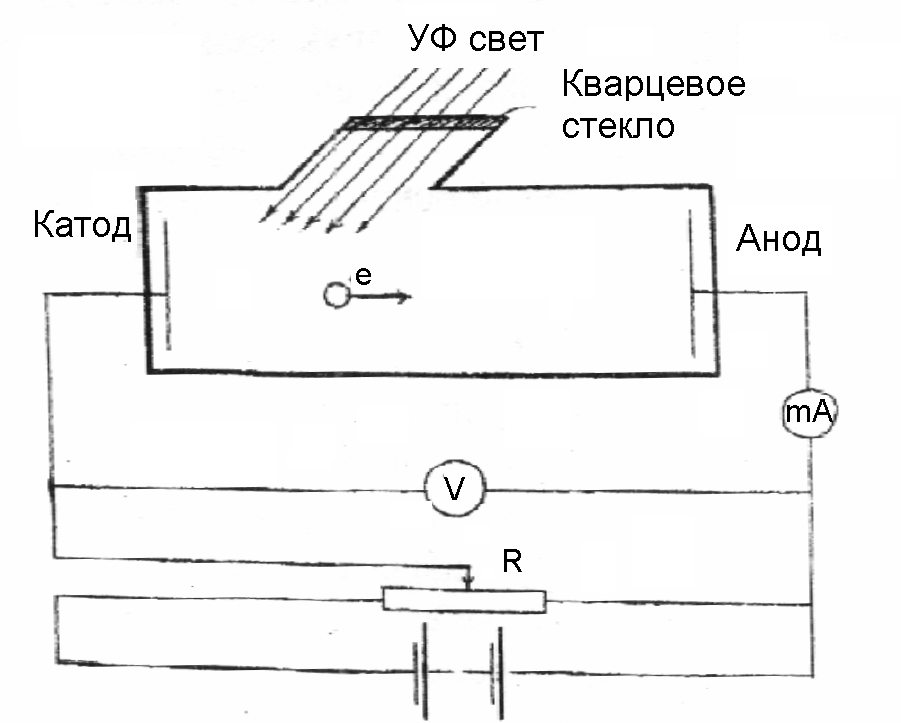
\includegraphics[width=1\linewidth]{pictures/2.png}
\caption{Схема эксперимента} %% подпись к рисунку
\end{minipage}
\hfill
\begin{minipage}[h]{0.3\linewidth}
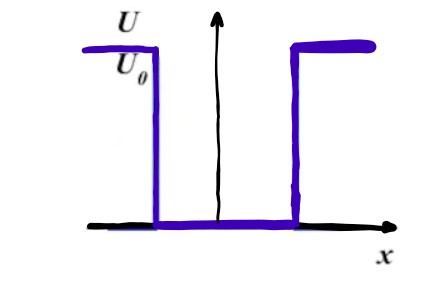
\includegraphics[width=1\linewidth]{pictures/2.1.jpg}
\caption{Потенциальный барьер}
\end{minipage}
\hfill
\begin{minipage}[h]{0.3\linewidth}
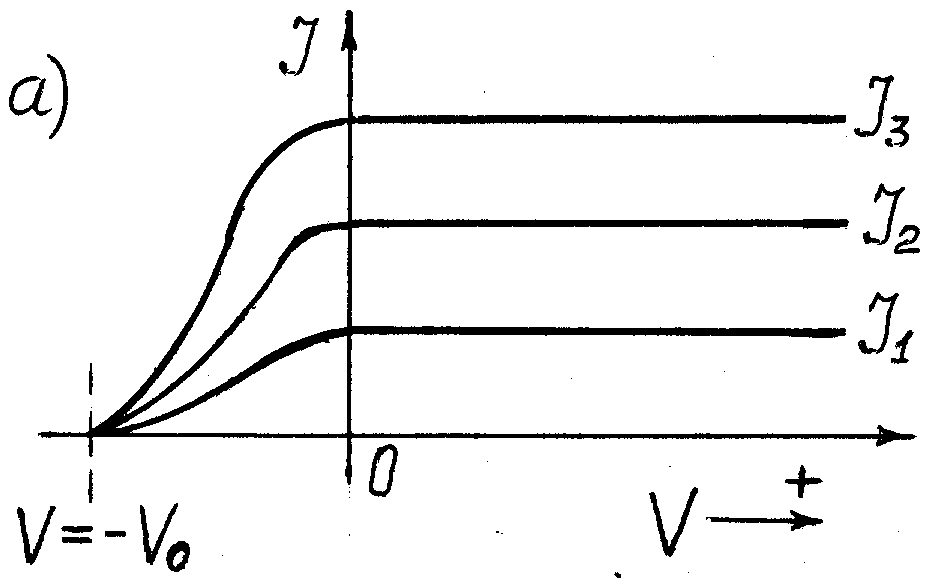
\includegraphics[width=1\linewidth]{pictures/2.2.png}
\caption{Зависимость фототока от напряжения}
\end{minipage}
\end{center}
\end{figure}


Но с точки зрения потенциала \textit{U} электрод - это ящик. Вообще есть и потенциалы атомов, действующих на этот электрод, забудем про них. Что бы вылететь, электронам необходимо преодолеть этот потенциальный барьер.
\par Пусть  $E \sim e^{i w t}$, тогда уравнение Ньютона будет выглядеть следующим образом (не забываем, что это грубая прикидка)
 $m a =e E_0 e^{i w t}$. Уравнение линейное, работать удобнее с комплексными экспонентами, в итоговом выражении возьмем действительную часть. Отсюда можем определить, что $v \sim e^{i w t}$, а ее амлитуда:
$$v_0 \simeq \frac{e E_0}{w m} \shortrightarrow E_{кин} = \frac{m e^2 E_0^2}{2m^2 w^2}=\frac{e^2 E_0}{2 m w^2} $$

\par Т.е. при низкой $w$ электроны быстро улетят, а поскольку приложено напряжение, потечет ток, но при облучении радиочастотной волной (от 3 кГц до 3000 ГГц) ничего не произойдет. На самом деле люди измеряют фототок как линейную функцию интенсивности $P=E_0^2$. С другой стороны, если измерить фототок в зависимости от поданного напряжения, то график окажется другим. Рассмотрим Рис.2.3, где три кривые обозначают три разные значения интенсивности: ток течет в случае $ I(V=0) \ne  0 $ (светим на определенный электрод, видимо, электроны там так выбились, что некоторые из них "на издыхании" долетели до 2 электрода, дали немножко тока), далее, прикладываем напряжение отрицательное, т.е. которое мешает движению частиц, лампа запирается, ток обращается в ноль. Запирающее напряжение не зависит от интенсивности облучения \textit{P}, что странно. Увеличивая  \textit{P}, мы увеличиваем количество выбитых электронов, рассмотрим $|U_0|$ как функцию частоты: она растет с некоторого порогового значения $w_п$- границы всего эффекта.

 \begin{wrapfigure}[12]{r}{0.4\linewidth} 
\vspace{-2ex}
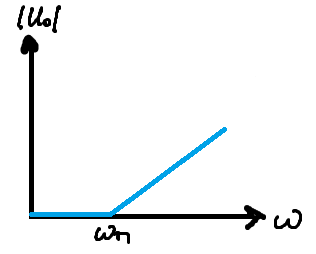
\includegraphics[width=0.7\linewidth]{pictures/2.3.png}
\caption{$|U_0|(w)$}
\end{wrapfigure}

 \par Запирающее напряжение в некотором смысле - мера энергии, которую мы сообщаем электрону при облучении, чтобы он вылетел, часть энергии может быть и остается, чтоб он куда-то летел. Эту самую избыточную энергию начинаем "душить", создавая противодействующую его движению туда. Запирание в этом смысле - явление, когда электрон мог преодолеть потенциальный барьер, но никуда не полетел, ток не пошел. Значит, существует какая-то красная граница фотоэффекта (т.к. для низких частот, а красный свет ниже всех по частоте). Вообще не понятно, почему это зависит от частоты, тем более таким образом.

\par Если свет может излучаться/поглощаться порциями (квантами) с энергией $E= \hbar w$, то ситуация получается простая: энергия, которую имеет квант света, тратится на некоторую величину, называемой работой выхода (это та самая величина потенциальной энергии, необходимая для преодоления барьера), вместе с остаточной кинетической энергией они связаны соотношением $\hbar w = A_e + E_k$. Энергия отсечки (когда кинетическая энергия обращается в ноль и ее не хватает для преодоления вышеупомянутого барьера) здесь такая, что $\hbar w \leq A_e $.

\newpage
\chapter{Излучение темного тела}
\section{Постановка проблемы}

\par Пусть у нас есть некий ящик длиной \textit{l}, нужно найти энергию поля $\rho (w) dw$, где $\rho(w)$ - спектральная плотность. Фактически, это энергия одной характерной моды, умноженная на число мод в интервале \textit{dw}. Разберём, как определить последнее. ЭМ поля представляют собой плоские волны: $\vec{E} \sim e^{i \vec{k} \vec{r}}$. Нас интересуют граничные условия (далее - ГУ) на стенках ящика. Уравнение на поле по пространственным производным - это уравнение второго порядка, поэтому нужно задать либо какое-то значение на стенках, либо значение производной. Но т.к. ящик очень большой, воспользуемся следующим приемом: ГУ наложим периодические
$$f(x+l,y,z)=f(x,y,z) $$
$$f(x,y+l,z)=f(x,y,z) $$
$$f(x,y,z+l)=f(x,y,z) $$
\par То есть получается наш ящик оказывается и не ящиком, а кольцом в 1D, тор - в 2D, тор четырехмерного пространства - в 3D. Данное описание весьма извращенное, но пока мы не интересуемся маленькими ящиками и не хотим думать о модах, которые будут связаны с ГУ на краях ящика (а они могут и быть), то в принципе все равно, какие ГУ накладывать. Конкретные значения $k_i$ дискретны, разные для каждого ГУ, но пока ящик большой, эта дискретность очень маленькая, почти непрерывна, поэтому нам совсем не важен вид ГУ. Подставляем трансляцию на размер ящика \textit{l} в экспоненту, чтобы периодичность сохранилась, фазовый множитель должен быть равен единице, тогда сама фаза $ 2 \pi n$:
$$ k_x l=2 \pi n_x$$
$$ k_y l=2 \pi n_y$$
$$ k_z l=2 \pi n_z$$
\par Небольшой обман: если разделить ящик пополам, поставить новую стенку, решить задачу предыдущую, получить новые ГУ на этой стенке, и здесь уже ГУ начальной задачи важны. Но для более-менее разумных ГУ (нулевые значения функции/производной) это не имеет значения, хотя всегда можно найти ГУ, когда все будет плохо.
\par Вообще \textit{n} - целые числа, а расстояния между соседними \textit{k} это $\frac{1}{l}$, а при $l \shortrightarrow \infty$ у нас $r \shortrightarrow 0$, k - практически непрерывен. В каком интервале  будем его считать? Дисперсионное уравнение дает модуль K есть $|\vec{k}|=\frac{w}{c}$. Если мы фиксируем какую-то \textit{w}, то в пространстве k мы фиксируем сферу радиуса k. Сделаем приращение $ k+d k$. Хотим сосчитать состояния в интервале (w, w+dw), т.е. нужно сосчитать количество дискретных точек K, находящихся между получившимися двумя сферами. 

\begin{wrapfigure}[18]{r}{0.4\linewidth} 
\vspace{-2ex}
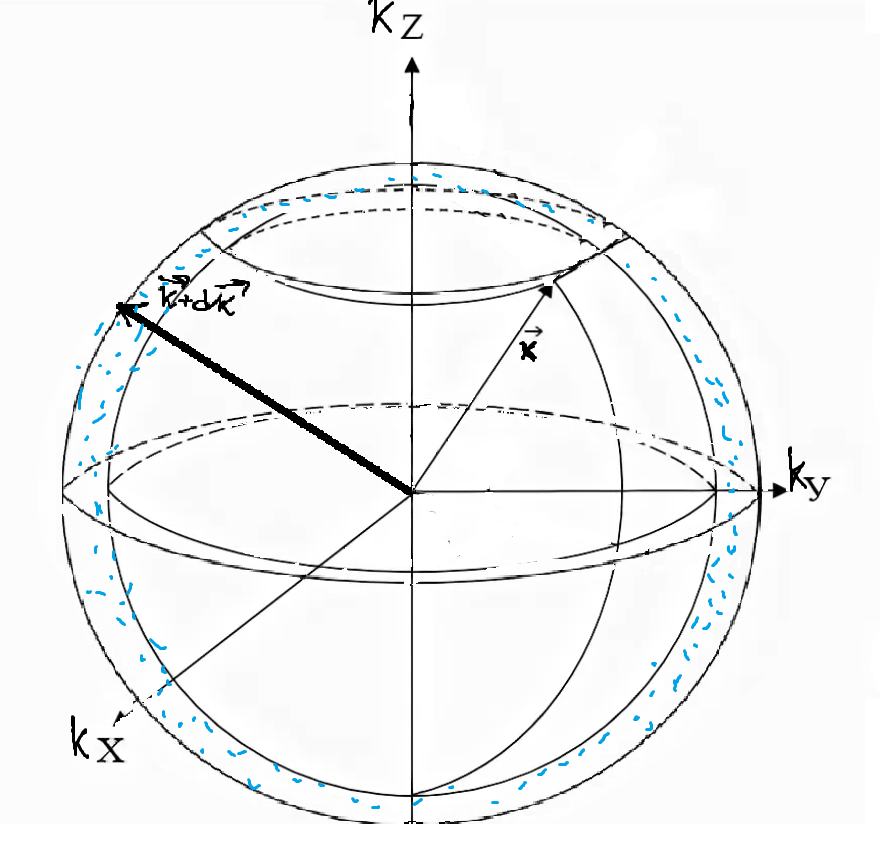
\includegraphics[width=1.2\linewidth]{pictures/3.2.png}
\caption{Координатное пространство k}
\end{wrapfigure}

 \par В нашем случае объем бесконечно малого слоя между сферами $V_{бм}=4 \pi k^2 \Delta k$ (площадь сферы, домноженная на толщину слоя). На каждую точку приходится маленький кубик со стороной $\frac{2 \pi}{l}$, нужно понять, сколько таких кубиков в сферическом слое. Для этого $V_{бм}$ делим на объем кубика \textit{V}. Нам не важно, что есть кубики, вылезающие за рамки слоя, т.к. они очень маленькие, имеют исчезающий размер, поэтому наш ответ верен в асимптотике  $l \shortrightarrow \infty$. Учитывая, что у волн есть 2 поляризации, имеем:
$$ dN = 2 \frac{4 \pi k^2 dk l^3}{(2 \pi)^3} =\frac{k^2dk V}{\pi ^2} $$
\par Подставим $k^2=(\frac{w}{c})^2$, получим $ dN_w =  \frac{w^2 V dw}{c^3 \pi^2} $. Мы сосчитали число колебаний, для поиска $\rho (w) dw$ считаем  $ dN_w $, деленная на единицу объема V и домножаем на некое среднее характерное значение энергии, которая приходится на одну моду $ \overline E_w$ (ибо мы имеем дело с термодинамикой, флуктуации нас не интересуют). Для определения этого среднего необходимо рассмотреть вероятность обнаружения молекулу в интервале скоростей [\textit{V}, \textit{V+dV}]: $f(V)d^3V$, где \textit{f(V)} - функция распределения. Когда имеем дело с термодинамическим равновесием, она имеет определенный вид, зависящий от температуры, хотя обычно обезразмеривают параметр, а так же принимают постоянную k=1: $f(\frac{E_к}{T})$. Распределение Гиббса (хотя вместо E обычно пишут H(p, q)):
$$ f \sim e^{-\frac{E}{T}} $$
$$\overline E_w = \int_{0}^{\infty} Ee^{-\frac{E}{T}}\,dE\ / \int_{0}^{\infty}e^{-\frac{E}{T}} \,dE\ $$
\par Это как бы энергия, взвешенная с числом состояний в интервале dE, а $e^{-\frac{E}{T}} dE$ - не число, а то, чему средняя энергия пропорциональна, поэтому нормируем на него, т.к. интеграл по всем инергиям даст нам единицу. Получим $\overline E_w = T$ (просто взяли интеграл). Закон Релея-Джинса
$$ \rho (w) = \frac{w^2 T}{\pi ^2 c^3} $$
\par Но если бы на сам деле $ \rho (w) \sim w^2 $, то тогда бы темное тело излучало: видимый свет, UV, рентгеновские лучи, $ \gamma $ излучение, но этого не происходит. Аналог темного тела - печь, но многие рядом с печкой находились и оставались живы. Почему?
\par 1896 г. Экспериментально был установлен закон Вина: на больших \textit{w} $$ \lim_{w\to\infty} \rho =e^{-\frac{b w}{T}} $$ В реальности интервал частот регулируется температурой (kT), поэтому существует ограничение полученной ранее несходимости, получившей название UV-катастрофы.



\section{Объяснение UV-катастрофы}

\par Планк утверждал, что проблема в расчете средней энергии моды. Предположение: \textit{E} может принимать только дискретные значения: $E=n E_0$, где \textit{n} - целое число, а $E_0$ что-то непонятное. Вероятность того, что частица имеет энергию $E_0$:   $e^{-n \frac{E_0}{T}}=e^{-n E_0 \beta}$, обозначение $ \beta = \frac{1}{T}$. ЭМ волны принимаются, поглощаются и излучаются стенками, причем это происходит только с дискретными энергиями. Далее вычислим среднюю энергию (в знаменателе сумма из условия нормировки, так же пользуемся суммой геометрической прогрессии):
$$ \overline E = \frac{\sum\limits_{n=0}^ \infty n E_0 e^{-n E_0 \beta}}{\sum\limits_{n=0}^ \infty e^{-n E_0 \beta}} = - \frac{d}{d \beta} ln \sum\limits_{n=0}^ \infty e^{-n E_0 \beta} = - \frac{d}{d \beta} ln \frac{1}{1- e^{-E_0 \beta}} = \frac{E_0}{e^{E_0 \beta} - 1}$$

\begin{wrapfigure}[14]{r}{0.4\linewidth} 
\vspace{-2ex}
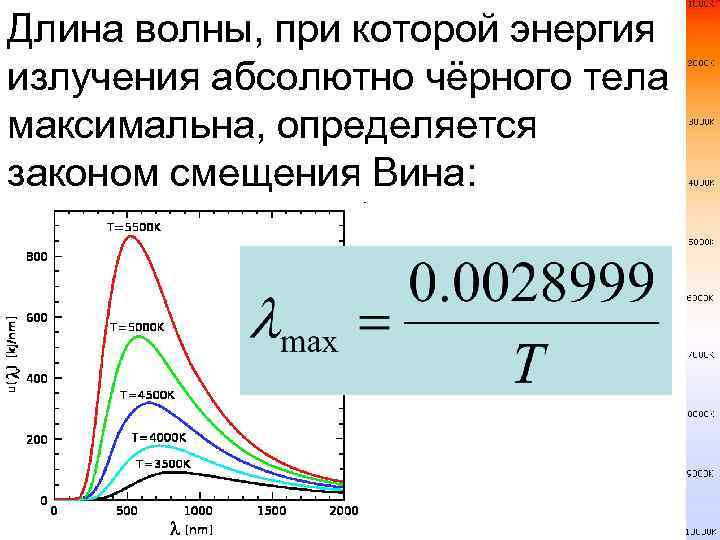
\includegraphics[width=0.8\linewidth]{pictures/3.3.jpg}
\caption{Закон смещения Вина}
\end{wrapfigure}

\par Гипотеза Планка $E_0 = \hbar w$. Видно, что при $ w \shortrightarrow \infty$ экспонента лидирует, получается закон Вина. Тогда при домножении $\overline E$ на число мод все будет хорошо. Из этих соображений можно подобрать $$ \hbar = 1,05 \cdot 10^{-27}эрг \cdot с $$
$$ h= 2 \pi \hbar $$
\par Отсюда $$ \rho (w) = \frac{1}{ \hbar ^2 c^3} \frac{\hbar w^3}{e^{\frac{\hbar w}{kT}}-1} $$ 
\par Максимум данного выражения по частоте наблюдается при $\frac{\hbar w_{max}}{T}=2.84$ (Закон смещения Вина). При низких частотах $ \hbar w < < T$ можно разложить $e^{\frac{\hbar w}{t}} \approx  1 + \frac{\hbar w}{T} $, тогда $ \rho (w) \approx \frac{1}{ \hbar ^2 c^3} \frac{\hbar w^3 T}{\hbar w} = \frac{1}{ \hbar c^3}  w^2 T $ - получили тот же самый ответ, что и раньше для малых частот (учитываем, что $E_0$ мало по сравнению с \textit{T}, а значит, суммирование заменяем интегрированием, т.к. функция на каждом шаге суммирования меняется очень мало). Для больших частот дело обстоит по-другому, как уже было сказано, в той области имеем экспоненциальное спадание, что тоже неплохо. 
\par В качестве развлечения посчитаем полную энергию, получим закон Стефана-Больцмана:
$$ U = \int_{0}^{\infty} \rho _w dw = \int_{0}^{\infty} \frac{1}{\hbar ^2 c^3} \frac{\hbar w^2}{e^{\frac{\hbar w}{T}}-1} dw = \frac{T^4}{\hbar ^2 \pi ^2 c^3} \int_{0}^{\infty} \frac{z^3 dz}{e^z -1} =\frac{T^4}{\hbar ^2 \pi ^2 c^3} \frac{\pi ^4}{15} = \frac{T^4 \pi ^2}{15 \hbar ^2 c^3}$$
\par Словесная формулировка: \textit{Энергия, излучаемая за единицу времени с единицы площади поверхности абсолютно черного тела во всем интервале частот от 0 до $\infty$, пропорциональна четвертой степени абсолютной температуры черного тела.} Вообще, примеров, когда температура контролирует частоту максимального излучения, немало. Сам Стефан применил свой закон к
излучению Солнца и определил температуру его поверхности - 5713 К (современное значение 5780 К, излучает оно больше в диапозоне зеленого света). Полученное им значение температуры Солнца оставалось самым точным в течение всего XIX века. 
\newpage
\chapter{Волна де Бройля. Волновые пакеты}
\par  В 1924 г. французский физик Луи де Бройль выдвинул смелую гипотезу, согласно которой корпускулярно-волновой дуализм имеет универсальный характер. Согласно его гипотезе каждая материальная частица обладает волновыми свойствами, причем соотношения, связывающие волновые и корпускулярные характеристики частицы остаются такими же, как и в случае электромагнитного излучения: \textit{"у каждой частицы есть некое поле, зависящее от $\vec{r}$, описывающее её, тогда можем это поле проквантовать (дискретизировать)"}. Т.е. с каждой частицей связана некая плоская волна какого-то комплексного поля $ \psi (\vec{r}, t) =\psi _0 e^{i \vec{k} \vec{r} - i w t} $.
\par Возникает вопрос, что это за неизвестная функция и как она связана с движением частицы. Чисто эмпирически были выявлены следующие соотношения, связывающие волновые и корпускулярные свойства частицы: $\vec{p} = \hbar \vec{k}$, $E= \hbar w$ (*). Вычислим фазовую скорость, т.е. скорость, с которой распространяются точки волны с постоянной фазой:
$$ v_ф = \frac{w}{k} = \frac{E}{p} = \frac{p^2}{2mp}= \frac{v}{2} $$
\par Вот и 1 неприятность: можем отказаться от уравнений Ньютона, понятия траектории и постулировать, что скорость частицы как раз \textit{v}, но это неправильно, ведь тогда придется отказаться от постулатов (*). Как быть? Во-первых, выражение для некой $ \psi (\vec{r}, t) $ патологично, ведь эта функция делокализована в пространстве полностью. Пока мы толком не знаем, что такое электрон, но по неведомым причинам в классической механике это то, что считается шариком, распространено во всем пространстве и по модулю в квадрате описывается функцией, которая сюда войти не может, что не исключено, но странно (??? Не понятно, что он вообще имел в виду).  Из соображения разумности хочется иметь описание, которое иногда приходило бы в движение шарика по орбите, иногда совершало бы какие-то чудеса (например, описывающее строение атома или еще что-нибудь), но эта функция не содержит ни намека на хороший переход к классике, т.е. не удовлетворяет ГУ. Как тогда с помощью $\psi$ проэмитировать движение частицы? Исправить ситуацию может собрание \textit{волнового пакета} - совокупности волн с разными импульсами (много фурье-гармоник), которую описывает волновая функция, заметно отличная от нуля только в очень малом участке пространства, размеры которого можно стремить к нулю вместе с $\hbar$. Если проинтегрировать в k-пространстве $\int_{k- \Delta k}^{k+ \Delta k} e^{ikx} dk = \frac{sin x}{x}$, а в реальном пространстве эта функция локализована. Рассматривая совокупность плоских волн с близкими k в каком-то интервале, соберем пространственный импульс, получим некоторую область, где $\psi$-функция в реальном пространстве не равна нулю в какой-то области, так же требуем, чтоб центр волнового пакета перемещался по истинной траектории классической частицы. Пробуем для простоты в 1D случае:
$$ \psi (x, t) = \int_{- \infty}^{\infty} с(p)  \psi _0 e^{\frac{i(px-E(p)t}{\hbar}} dp $$
\par Нормировка: $$\int | \psi |^2 dx = \iint dp \, dp^\prime c(p)c(p^\prime) | \psi _0 |^2 e^{\frac{i(E\prime-E)t}{\hbar}}  \underbrace{\int e^{\frac{i(p-p^\prime)x}{\hbar}} dx}_{\text{а это } 2 \pi \hbar \delta (p-p^\prime)}=  2 \pi \hbar  | \psi _0 |^2 \int |c|^2 dp $$
\par 
\begin{wrapfigure}[11]{r}{0.3\linewidth} 
\vspace{-2ex}
\centering
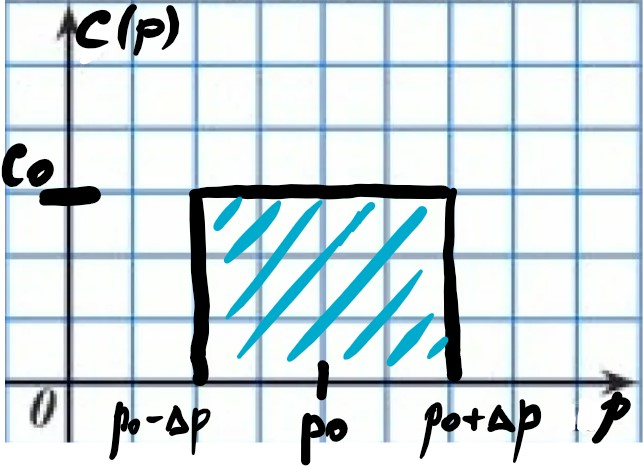
\includegraphics[width=0.8\linewidth]{pictures/4.1.jpg}
\caption{Выбор константы}
\end{wrapfigure}
\par Подберем
$ \psi _0 =\frac{1}{\sqrt{2 \pi \hbar}} $, дальше, если подобрать правильное поводение \textit{с} на $\infty$, можем обеспечить регулярный характер поведения этой нормы. Предположим, что зависимость такая: $c_0 = 1, p \in (p_0- \Delta p, p_0 + \Delta p ) $. Раскладываем вблизи $p_0$ энергию и ищем волновую функцию:
$$ E(p)= E_0 + (p-p_0) \frac{dE}{dp} \bigg|_{p=p_0} $$
$$ \psi = c_0 \int_{p_o - \Delta p}^{p_o + \Delta p} \frac{1}{\sqrt{2 \pi \hbar}} e^{\frac{i(px-Et)}{\hbar}} dp =\bigg| p=p_0+ \hbar \xi \bigg| =\frac{c_0 \hbar}{\sqrt{2 \pi \hbar}} e^{\frac{i(p_0x-E_0t)}{\hbar}} \int_{\frac{ - \Delta p}{\hbar}}^{\frac{ \Delta p}{\hbar}} \,e^{i \xi (x- \frac{dE}{dp})|_{p=p_0} t } \, d \xi =$$
$$=\frac{c_0 \hbar}{\sqrt{2 \pi \hbar}} e^{\frac{i(p_0x-E_0t)}{\hbar}} \cdot 2 \frac{sin(\Delta p) (x- \frac{dE}{dp}|_{p=p_0} t )}{\hbar (x- \frac{dE}{dp}|_{p=p_0} t )} $$
\par Получилась функция $\frac{sin(\frac{\Delta p \chi}{\hbar})}{\chi}$, которая локализована вблизи $\Chi = 0$, т.е. центра масс пакета движется с групповой скоростью (максимум функции при любых временах лежит в одной точке) $x=\frac{dE}{dp}|_{p=p_0} t = \frac{p_0 t}{m} = v_0 t $ равномерно, что не противоречит II закону Ньютона ($ \dot{v} =0$) в отсутствии действия внешней силы). Что отсюда важного стоит извлечь: у этого пакета есть ширина, а сама функция отлична от нуля, когда ее аргумент </порядка 1: $ \frac{\Delta p \cdot \Delta x}{\hbar} \sim 1 $. Т.е. пакет движется примерно по классической траектории частицы, но при этом точность определения ее зависит от точности определения импульса: при размывании $\Delta p$ размывается и $\Delta x$. Возникает соотношение неопределенности $ \Delta p \cdot \Delta x \sim 2 \pi h $
\par Энергия связана с импульсом, мы предполагали, что $E \sim e^{-iwt} $, а значит, если посчитать то же самое при $p^2 $, пакет "расплывётся".
 
\newpage
\chapter{Физический смысл волновой функции в квантовой механике}
 
\begin{wrapfigure}[12]{r}{0.4\linewidth} 
\vspace{-2ex}
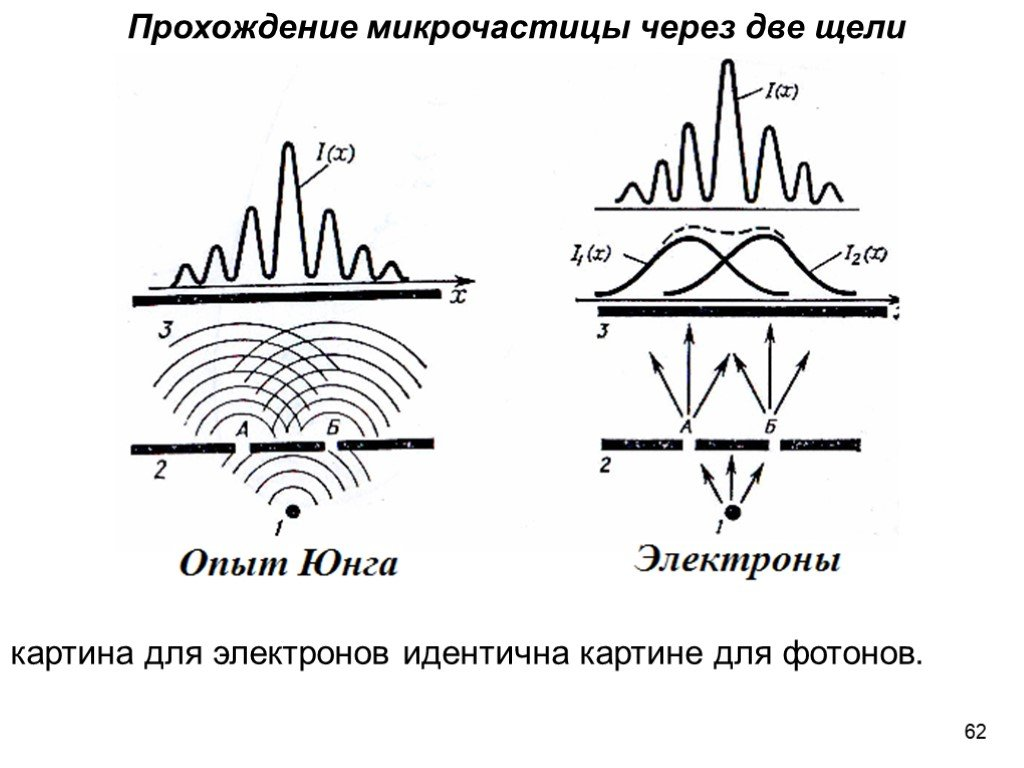
\includegraphics[width=0.9\linewidth]{pictures/4.2.jpg}
\caption{Схема эксперимента}
\end{wrapfigure}
\par Проведем мысленный эксперимент: пусть есть два экрана, первый из которых имеет два отверстия. Если же разместить перед экранами источник света, мы увидим ожидаемую интерференционную картинку, даже если закроем одно из отверстий. Заменим теперь источник света на источник электронов и зафиксируем наблюдения: если отверстия закрывать по очереди и посмотреть, какая картина будет суммарной, то получится совсем другой результат. Вывод: в некотором смысле частицы ведут себя точно так же, как волны, но вне зависимости от того, один электрон полетит или сразу пучок, при помещении лампочки перед экранами, картинка полностью пропадает. 
\par Пусть летит 1 электрон. Но интерференция не имеет место в данном случае, получается крайне идиотская ситуация - один и тот же электрон идет и через 1ое отверстие, и через второе сразу. Поставим еще лампочку перед 2 экраном - картинка пропадет совсем, даже если "стрелять" по одному электрону. Лампочка здесь играет роль некого источника ЭМ излучения, она позволяет увидеть (значит, измерить) рассеянное излучение - рассеяние частицы, но ведь выяснять уже нечего, т.к. картинки нет.
\par Значит, мы должны строить описание в терминах некой функции распределения $P(\vec{r})$, т. ч. интеграл по объему даст вероятность увидеть эту частицу в данном объеме. В оптике или волновой теории необходимо описание в терминах амплитуды и фазы волны, значит, требуется некая комплексная функция $ \psi (\vec{r}, t)$ и уравнение на нее. Знаем, что $|\psi (\vec{r}, t)|^2 d^3r$ может представлять собой вероятность (это действительная величина), так же $\psi$ предполагает взаимодействие с классическим прибором для понимания определения этой функции - \textit{волновой функции (комплексной амплитуды)}. Другими словами, посмотреть на электрон мы не можем, т.к. при отсутствии измерений нет и явлений, а при измерении прибором состояние сразу меняется. (О проблеме квантово-механического описания лучше не задумываться)
\par Пусть движение электрона через 1 отверстие описывает комплексная амплитуда $\psi _1$, а через второй - $\psi _2$ (хотя на самом деле стоит вводить целое множество, поговорим хотя бы про 2). Классические пути при столкновении с экраном интерферируют, на последнем экране видим фактически их сумму $c_1 \psi _1 + c_2 \psi _2 $, тогда взяв $ |c_1 \psi _1 + c_2 \psi _2 |^2$, получим распределение. Фазы комплексных функций будут зависеть от конкретных точек наблюдений. Анализируя эксперимент, мы должны складывать не вероятности прохождения, а комплексные амплитуды.
\par
\par В классической механике движение происходит по траектории, отвечающей минимуму функционала действия, а квантомеханическая частица может двигаться по различным траекториям (все они равновероятны), причем одновременно. В пустом пространстве (без экранов и отверстий) все так же. Частица идет сразу по всем траекториям, каждой из которых соотвествует некая $\psi$, результатом брать сумму всех таких пси по модулю в квадрате. В реальности частиц множество, как все устроено, если $\psi (\vec{r_1}, \vec{r_2}) $?
\par
\begin{wrapfigure}[12]{l}{0.3\linewidth} 
\vspace{-2ex}
\centering
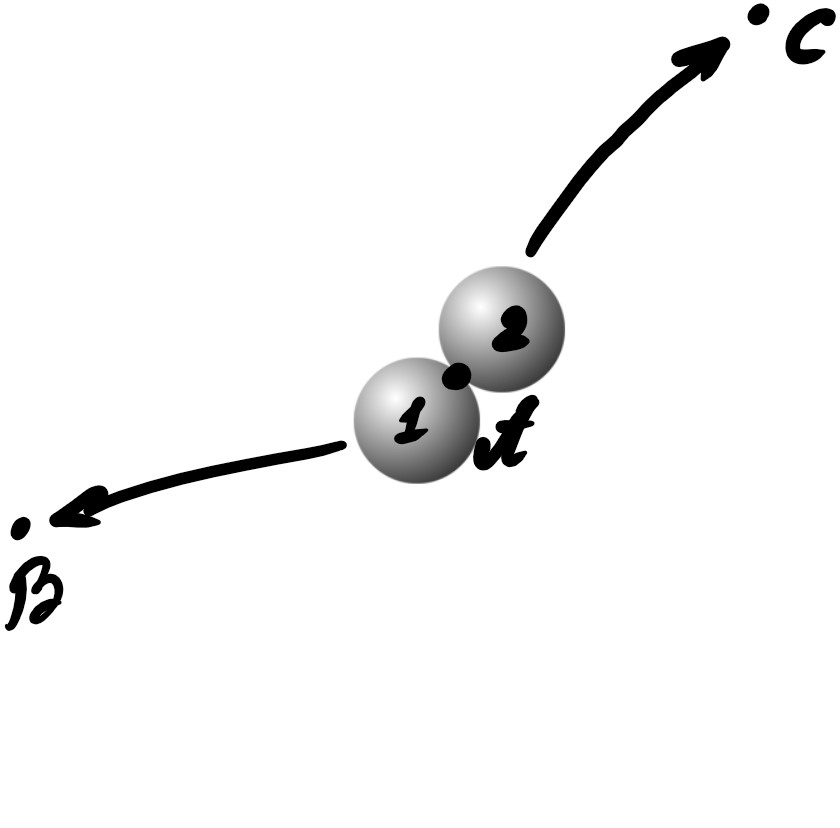
\includegraphics[width=0.8\linewidth]{pictures/5.2.jpg}
\caption{Иллюстрация к тексту}
\end{wrapfigure}
\par Практически постулат: пока частицы не взаимодействуют, можем искать волновую функцию как $ \psi _1 (\vec{r_1}) \cdot \psi _2 (\vec{r_2})$. Это автоматически означает, что  в уравнениях эти частицы подразумевают разделение переменных в таком пределе, т.е. они должны быть линейные. Допустим, в точке А было определенное состояние двух квантовомеханических частиц, их отпустили, частицы разлетелись далеко друг от друга. Проводя измерения в точке В, мы одновременно определим состояние $2^{ой}$ частицы в т. С, т.к. $\psi$ - общая.
\par Такая трактовка означает, что имеет место коллосальная степень нелокальности. При таком взгляде на вещи скорость света - не предел, но если мы измеряем что-то реальное, то расчеты дадут разумный результат, т.е. в ответах подобных пародоксов не возникает. 
\newpage
\chapter{Операторы физических величин и их собственные значения}

\par Пусть у нас имеется несколько классических приборов, измеряющих некую физическую величину. Обозначим её \textit{f}, каждой такой величине ставится в соответствие оператор $\hat{f}$, который может действовать на волновую функцию $\psi$. Процесс измерения заключается в том, что классический прибор и частица приходят во взаимодействие друг с другом, в результате чего прибор переходит из начального в некоторое другое состояние, и по этому состоянию мы судим о состоянии частицы. Описание состояний прибора осуществляется квазиклассическими волновыми функциями. Тогда в результате измерения величины \textit{f} получим набор собственных значений $f_n$:
$$ \hat{f} \psi _n (\vec{r}, t) = f_n \psi_n $$
\par С другой стороны, на вход прибора совершенно не обязательно приходит собственная функция, может быть и суперпозиция с некоторыми коэффициентами разложения, т.е. с прибора мы снимаем среднее значение величины \textit{f}, а значит в каждом конкретном измерении получаем какое-то одно $f_n$, не меняя условий эксперимента и возвращая частицу к начальному состоянию, повторяем многократно, а затем усредняем результат:
$$ \overline{f} = \int \psi ^* \hat{f} \psi d^3r =  \int \psi ^* \hat{f} \psi dq$$
\par Условие нормировки $\int |\psi|^2 dq = 1$ (т.к. речь идет о вероятности найти частицу хоть где-то, о классе функций). Но так хорошо работать только с дискретным спектром собственных значений $f_n$, т.к. функция хорошо локализована в пространстве и интеграл существует. С непрерывным спектром оператора есть некоторые тонкости, о которых пока не будем  говорить. Можно себя успокаивать так: любую частицу можем закрыть в ящике, где нормировка может быть осуществлена.
\par Конкретизируем аксиоматику (написать уравнение на волновую функцию, установить правила определения операторов физ. величин). Получить операторы физических величин нельзя, но можно ввести их, учитывая, что в конкретных пределах не должно быть отличия от классики. Начнем с вида волновой функции.

\begin{wrapfigure}[8]{l}{0.25\linewidth} 
\vspace{-2ex}
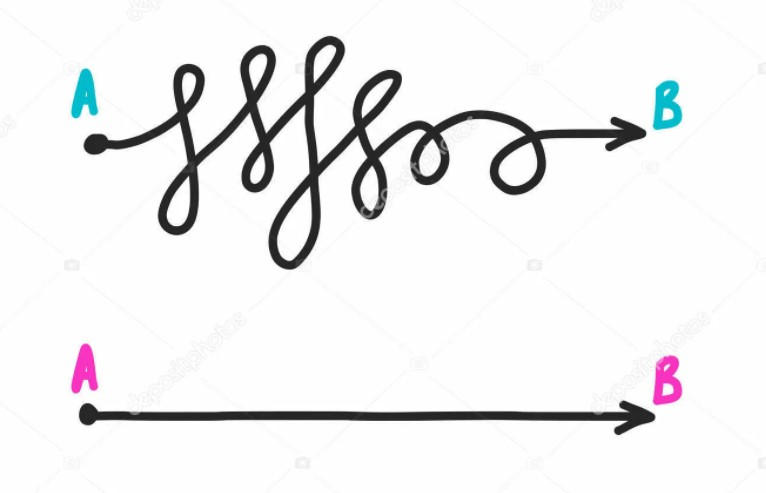
\includegraphics[width=1.1\linewidth]{pictures/5.1.jpg}
\caption{Иллюстрация к принципу Ферма}
\end{wrapfigure}

\par В качестве классического предела для волновой функции рассмотрим $\psi \sim e^{i \frac{S}{\hbar}}$, где \textit{S} - действие, эйконал. Все это представление должно срастить с уравнениями Ньютона, т.е. с экстремумом действия \textit{S}. Для света длину оптического пути можно найти из принципа Ферма: свет выбирает из множества путей между двумя точками тот путь, который потребует наименьшего времени (по лучу). А значит, требуется найти минимум функционала $ S = \int_{A}^{B} n dl$, где $n = \sqrt{\varepsilon}$ - показатель преломления. Как это получить из уравнений Максвелла? $ \frac{\varepsilon}{c^2} \frac{\partial ^2 }{\partial t ^2} \vec{A} = \underbrace{- \frac{4 \pi}{c} \vec{j}}_{\text{какие-то источники}} $. Векторный потенциал с полями связаны следующим образом:
$$\vec{B} = rot \vec{A} $$
$$ \vec{E} = - \frac{1}{c} \frac{\partial \vec{A}}{\partial t} - \nabla \varphi$$
\par То, о чем мы говорим - приближение, которое верно при определенных условиях (ведь то, что свет пойдет по лучу - тоже приближение, не учитывающее дифракцию и интерференцию). Пусть \textit{n} однородно, тогда ищем решения уравнения Максвелла в виде $e^{-iwt +i \vec{k} \vec{r}}$. Свет распространяется вдоль вектора $\vec{k}$, это и есть лучи из принципа Ферма. Можем попробовать искать поля $\vec{E}, \vec{B} \sim \vec{a} \cdot e^{i \varphi}$:
$$ \frac{\partial \varphi}{\partial t} = -w $$
$$ \frac{\partial \varphi}{\partial \vec{r}} = \vec{k} (\vec{r}) $$
\par Откуда $$ \varphi = -wt + \frac{\epsilon w}{c} \varphi_1 $$
$$ (\nabla \varphi _1)^2 =n^2 (x,y,z) \Longrightarrow \varphi_1 = \int n dl $$
\par Где $\varphi_1$ играет роль эйконала, а интегрирование ведется вдоль луча. Линии градиента можем воспринимать как эти лучи, они имеют смысл локального вектора $\vec{k}$. $rot(\nabla \varphi_1)=0 \longrightarrow $ получим решение, которое работает, если масштаб изменения свойств среды $L(n) >> \lambda$. (В лучевой $\lambda \approx 0$, а масштабы искривления много больше) Приближение геметрической оптики здесь называется \textit{эйкональным приближением}.

\begin{table}[h]
\centering
\begin{tabular}[c]{|c|c|}
\hline 
Оптика & Хотим аналог в квантах \\ \hline 
Эйконал S & Действие S \\
$\varphi, \vec{A} \sim e^{iS} $ & $\psi \sim e^{i \frac{S}{\hbar}}$ \\
лучи & траектории по Ньютону \\
принцип Ферма & принцип Мопертюи \\
$dS =-w dt + \frac{w}{c} \vec{k} d\vec{l}$ & $dS=-Hdt+ \sum_{i}p_idq_i$ \\
\hline
\end{tabular}
\end{table}
\par Из теоретической механики знаем, что для нахождения минимума функционала действия, нужно проварьировать его и приравнять первую вариацию к нулю:
$$\delta S = \sum_{i} \frac{\partial L}{\partial \dot{q_i}} \delta q_i \bigg|_{t_1}^{t} + \sum_{i} \int_{t_i}^{t} \underbrace{ \bigg( \frac{\partial L}{\partial q_i} - \frac{d}{dt} \frac{\partial L}{\partial \dot{q_i}} \bigg) }_{\text{для классической механики ноль}} \delta q_i dt $$
$$ \delta q_i(t_1)=0 \Longrightarrow \delta S = \sum_{i} p_i \delta q_i $$
$$ \frac{dS}{dt} = \frac{\partial S}{\partial t} +\sum \frac{\partial S}{\partial q_i} \dot{q_i} = \frac{\partial S}{\partial t}+ \sum p_i \dot{q_i} \Longrightarrow \frac{\partial S}{\partial t} = L -  \sum_{i} p_i \dot{q_i}= -H  $$
\par По аналогии с оптикой хочется, чтоб выполнялся закон сохранения энергии $E=H \Longrightarrow S = \underbrace{\int \sum p_i dq_i}_{\text{укороченное действие }S_0} - E(t-t_0)$. Для материальной точки в 3D, например, $p=\sqrt{2m(E-U)}$, $$S_0 = \int \vec{p}d \vec{r}=\int \sqrt{2m(E-U(\vec{r}))} dl $$
\par Назовем подынтегральное выражение показателем преломления n и получим аналог принципа Ферма - \textit{принцип Мопертюи}.
\par В уравнении на $\psi$ желательна некая линейность (ради выполнения принципа суперпозиции), рассмотрим:
$$ \frac{\partial \psi}{\partial t} =\frac{\partial}{\partial t} ( e^{i \frac{S}{\hbar}} ) = \frac{i}{\hbar} \frac{\partial S}{\partial t} \Psi =  \frac{i}{\hbar} (-H) \psi$$
\par Так называемое уравнение Шрёдингера
$$ i \hbar \frac{\partial \psi}{\partial t} = H \psi $$
\par Теперь отказываемся от идеи $\psi \sim e^{\frac{iS}{\hbar}}$, запишем оператор Гамильтониана $$\hat{H} = \frac{\hat{\vec{p}}^2}{2m}+U(\hat{\vec{r}})$$
\par Осталось определить, что есть оператор импульса и координаты и  \colorbox{orange}{как они действуют на $\psi$.}
$$ \hat{\vec{p}} \psi = \nabla S \psi  \Longrightarrow \hat{\vec{p}} = -i \hbar \nabla  $$
\par Уравнение без источника, значит, нужны условия на $\psi$:  $\psi \ne 0 $ + условие нормировки $\int |\psi|^2 d^3r = 1$. Продифференцируем последнее соотношение по времени:
$$ \int dq (\dot{\psi} \psi^{*} +\psi \dot{\psi^{*}}) = \int dq ( \psi^{*} \frac{\hat{H}}{i \hbar} \psi - \psi \frac{\hat{H^*}}{i \hbar} \psi^*) =\frac{1}{i \hbar} \int \psi^*\hat{H} \psi dq - \underbrace{\frac{1}{i \hbar} \int \psi^*\hat{\widetilde{H}} \psi dq}_{\text{здесь поменяли местами } \psi^* \text{ и }\psi} = 0 $$
\par Здесь $\hat{\widetilde{H}}$ - транспонированный оператор, $\hat{\widetilde{H}}^* = \hat{H}^+$ - оператор, эрмитово сопряженный исходному. Для выполнения верхнего равенства требуем эрмитовость оператора гамильтониана $\hat{H}=\hat{H}^+$ ($\forall \psi$). 
\par \textit{Небольшое отступление. Все ли операторы физических величин эрмитовы? Рассмотрим оператор импульса} $\hat{\vec{p}} = -i \hbar \nabla$: определению соответствует $$ \int \psi_1 \hat{\vec{p}} \psi_2 dq = -i \hbar \int (\underbrace{\nabla (\psi_1 \psi_2)}_{\text{Хотим ноль на }\infty} - \psi_2 \nabla \psi_1) dq = \int \psi_2 (i \hbar \nabla)\psi_1 dq \Longrightarrow \hat{p}^т=-\hat{p} $$
$$ \hat{p}^+ = -\hat{p}^* = \hat{p} \text{- эрмитов}$$
\par \textit{Для вычисления любой величины требуется найти среднее: $\overline{f}=\int \psi^* \hat{f} \psi dq$. Показания классического прибора должны быть действительными} $ \overline{f} \in \mathbb{R}$. 
$$ \overline{f^*}= \int \psi \hat{f^*} \psi^* dq = \int \psi^* \hat{f^+} \psi dq$$
\par \textit{Это выполняется $\forall \psi$, следовательно, $\hat{f^+} = \hat{f}$.}

\par Итак, хотим найти собственные функции оператора импульса $ \hat{\vec{p}} \psi_p = \vec{p} \psi _p $, фактически, мы раскладываем $\psi_p$-функцию по базису из собственных функций оператора $\hat{\vec{p}}$, получаем $\psi_p \sim e^{\frac{i\vec{p}\vec{r}}{\hbar}}$ - плоские волны.
\par Оператор координаты - это домножение на нее: $\hat{x} \psi = x_0 \psi$, собственной функцией данного оператора является $\delta$-функция. (Вообще именно поэтому мы не можем перейти от одного к другому, от $\delta$-функции к плоским волнам: $[\hat{x}\hat{p}]=i\hbar$)
\par Теперь рассмотрим оператор параллельного переноса $\hat{T}_{\vec{a}} \psi (\vec{r}) = \psi ( \vec{r} + \vec{a} )$. Для этого разложим $\psi (\vec{r}+\vec{a})$ в ряд Тейлора и заменим производную по r на известное нам действие оператора $\hat{\vec{p}}$ с соотвествующими коэффициентами:
$$\psi (\vec{r}+\vec{a}) = \psi (\vec{r}) + \vec{a} \frac{\partial}{\partial r} \psi + ... = (1+\frac{i}{\hbar}(\vec{a}\hat{\vec{r}}) + \frac{1}{2}(\frac{i}{\hbar}(\vec{a}\hat{\vec{r}})^2) +...)\psi $$
\par Получим $$\hat{T}_{\vec{a}} = e^{\frac{i}{\hbar}\vec{a}\hat{\vec{r}}}$$

\newpage
\chapter{Операторы физических величин и матрицы}
\par Примеры операторов физических величин рассмотрены в предыдущем вопросе.
\section{Матричная формулировка квантовой механики}
\par Если мы фиксируем какое-то представление, а это представление дискретно в том смысле, что мы раскладываем по собственным функциям дискретного спектра, то каждому оператору в этом представлении можем поставить в соотсествие некоторую матрицу.
\par Пусть есть разложение произвольной $\psi$-функции по некоторому базису (с коэффициентами) - полному дискретному набору собственных функций какого-то оператора - $\psi = \sum_{n} a_n\psi_n$, для перехода к новому представлению необходимо верно определить вычисление средних. Несложно видеть, что общее определение может быть записано в следующем виде:
$$\overline{f}=\sum_{nm}a^*_n a_m f_{nm}(t) $$
\par  Причем матричный элемент $f_{nm}(t) = \int \psi^*_n \hat{f}\psi_m dq = f_{nm}e^{iw_{nm}t}$, здесь частота перехода $w_{nm}=\frac{E_n -E_m}{\hbar}$, а $f_{nm}=\int a^*_n \hat{f}\psi_m dq$. Предполагаем, что функции $\psi_n$ и $\psi_m$ соответствуют определенным энергиям, тогда на каждой "сидит" временная экспонента $ \sim e^{\frac{i E_j}{\hbar}} $, которую спокойно вынесли из-под интеграла.

\begin{remark}
\par \textit{Почему можем сказать, что формула записана в представлении Гейзенберга? Вернемся к общему определению среднего. Здесь $a^*_n$ и $ a_m$ играют роль волновой функции (мы так это записали, ввели без зависимости от времени), а вся зависимость от времени "сидит" \, в матрице $f_{nm}$, которая теперь играет роль оператора. В этом смысле запись пободна представлению Гейзенберга, но мы могли бы сделать и по-другому: временную зависимость "отправить"\, в $a^*_n$ и $ a_m$, получили бы некоторое другое выражение, но в том же духе. То есть этот экспоненциальный фактор можно либо оставить на матрице f, либо отправить на коэффициенты, это сейчас не важно.}
\end{remark}
\par Получившуюся \textit{f} естественно называть матрицей физической величины \textit{f}. Как определить производную по времени? Как и раньше, через производную по времени от среднего \textit{f}:
$$\overline{{\dot{f}}} = \dot{\overline{f}} = \sum_{mn} a^*_n a_m \dot{f}_{nm}(t) $$
\par где $\dot{f}_{nm}(t) = i w_{nm} f_{nm}(t)$. 
\begin{remark}
\par \textit{Что было бы с $f_{nm}$, если бы мы работали в базисе собственных функций оператора $\hat{f}$? Естественно, была бы диагональной, но мы этого не предполагаем.}
\end{remark}
\par Можем определить матрицу жрмитово сопряженного оператора, используя определение транспонированного оператора: $(f^*)_{nm} = \int \psi^*_n \hat{f^*}^T \psi_m dq = \int \psi_m f^* \psi^*_n dq$. Тогда
$$(f^*)_{nm}=(f_{mn})^*$$
\par Для вещественной физической величины $f_{nm}=f^*_{mn}$.
\section{Умножение матричных операторов}
\par Как с точки зрения матриц устроено умножение операторов? Распишем действие оператора на волновую функцию:
$$\hat{f} \psi_n = \sum_{m} f_{mn}\psi_{m}$$
\par А теперь рассмотрим действие произведения операторов, используя вышеприведенную формула сначала для оператора $\hat{g}$ и "протаскивая" \, оператор $\hat{f}$ (ведь он действует на волновую функцию), а потом и для $\hat{f}$:
$$\hat{f} \hat{g}\psi_n = \hat{f} \sum_k g_{kn}\hat{f}\psi_k = \sum_{km}g_{kn}f_{mk}\psi_m = \sum_m (fg)_{mn} \psi_m$$
\par Причем $f_{mk}g_{kn} = (fg)_{mn}$ - обычное матричное произведение. Пусть у нас есть задача на поиск собственных значений некоторого оператора $\hat{f}$: $\hat{f}\psi = f\psi$. Подставим разложение собственной функции $\psi = \sum_m C_m \psi_m$, тогда получим:
$$\sum_m C_m \hat{f} \psi_m = f \sum_{m}C_m \psi_m$$
\par Скалярно домножим на $\psi^*$ и проинтегрируем по пространству. Результат: 
$$ \sum_m f_{nm} C_m = f C_n$$
\par Как видно, задача на поиск собственных значений в матричном представлении сводится к вычислению собственных значений и векторов матрицы \textit{f}. Согласно линейной алгебре, для существования нетривиального решения (т.к. есть линейно зависимые строки)
 $det(f_{nm}-f_m\delta_{nm})=0 \rightarrow $ получим некоторое количество собственных значений. В базисе собственных функций матрица диагональна и представима в виде:  $f_{nm}=f_m\delta_{nm} $. Часто используют \textbf{обозначения Дирака}:
$$ f_{nm} \equiv < n|f|m> $$
$$ <n|m> = \int \psi^*_n \psi_m dq $$
\section{След и его свойства (полезное дополнение)}
\par \textbf{След матрицы} - это сумма всех ее диагональных элементов. Обозначается как \textbf{Sp} (от нем. \textit{Spur} — след) или \textbf{tr} (от англ. \textit{trace} — след).
\par 1\textdegree. $Spf=\sum_n f_{nn}$
\par 2\textdegree. $Sp(\hat{g}\hat{f})=Sp(\hat{f}\hat{g})$
\par 3\textdegree. $Sp(abc)=Sp(cab)$

\newpage
\chapter{Условие нормировки для волновых функций. Непрерывный и дискретный спектр}
\par Рассмотрим нормировку собственных функций непрерывного спектра на примере оператора импульса: $\hat{\vec{p}} \psi_p = \vec{p} \psi_p$. Под спектром всегда имеем в виду спектр собственных значений какого-то оператора.
$$ -i \hbar \nabla \psi_p = \vec{p} \psi_p $$
$$ \psi_p \approx  e^ \frac{i \vec{p} \vec{r}}{\hbar} $$
\par Фактически, волновую функцию раскладываем по базису из СФ оператора $\hat{\vec{p}}$. Итак, пусть есть некая физическая величина \textit{f} с СФ $\psi_f$: $\hat{f}\psi_f = f \cdot \psi_f$, нашли мысленно все орты в функциональном пространстве, перешли в f-представление, предполагая, что спектр непрерывный, тогда: $\psi (q)= \int a_f \psi_f df$, \textit{q} - обобщенная координата. Это \textbf{общее устройство смены представления}. Хотим нормировку, характерную для плотности вероятности: $\int \psi \cdot \psi^* dq = \int |a_f|^2 df =1$.
$$ \int \psi \cdot \psi^* dq = \iint a_f^* \psi_f^* \psi df dq \longrightarrow a_f = \int \psi(q) \psi_f^*(q) dq$$
\par Подставим представление $\psi (q)$ в полученную формулу для $a_f$: 
$$ a_f = \int a_{f\prime} \underbrace{\bigg( \int \psi_{f\prime} \psi_f^* dq \bigg)}_{\text{должно быть } \delta(f- f\prime)} df\prime $$
\par Возвращаемся к представлению $\psi (q)$:
$$ \psi (q) = \int \psi(q\prime) \underbrace{\bigg( \int \psi_f^*(q\prime) \psi_f (q) df \bigg)}_{\text{еще условие } \delta(q- q\prime)} dq\prime $$
\par Так же это называется \textit{ условием полноты}. Если полный спектр дискретен, то $\sum_{n} \psi_n^* (q\prime) \psi_n (q)= \delta(q- q\prime)$. Итого условие нормировки: 
$$ \int \psi_{p\prime}^*  \psi_p d^3r = (2 \pi \hbar) ^3 \delta (\vec{p\prime} - \vec{p})$$
$$ \psi(\vec{r}) = \int a(\vec{p}) \psi_p (r) \frac{d^3 p}{(2 \pi \hbar)^3} \text{, где }  a(\vec{p}) =\int \psi(\vec{r}) e^{-\frac{i \vec{p} \vec{r}}{\hbar}} d^3r $$
\par Вероятность того, что частица попадет в интервал импульса $d^3p$ есть $|a(\vec{p})|^2 \frac{d^3 p}{(2 \pi \hbar)^3} $, здесь используется свойство $\delta$-функции:
$\frac{1}{2 \pi} \int e^{i \alpha x} d \alpha = \delta (x)$.
\par Повторим предыдущие рассуждения для дискретного спектра:  $\hat{f}\psi_n = f_n \cdot \psi_n$, разложим по системе СФ $\psi = \sum_{n} a_n \psi_n$, требуем $\sum_{n}a_n a_n^* =\int \psi^* \psi dq =1 $. Домножим скалярно справа на волновую функцию выражение  $\psi^* = \sum_{n} a_n^* \psi_n^*$ и проинтегрируем по \textit{dq}:
$$ \int \psi^* \psi dq = \sum a_n^* \int \psi_n^* \psi dq \rightarrow a_n = \int \psi \cdot \psi_n^* dq$$
\par Подставим разложение для волновой функции:
$$ a_n = \sum_{m}a_m \int \psi_m \psi_n^* dq$$
\par Для выполнения условий требуем $\int \psi_m \psi_n^* dq = \delta_{nm}$
\newpage
\chapter{Непрерывный и дискретный спектр. Вырождение уровней}
\par По определению о \textit{вырождении уровней} говорят, если одному собственному значению оператора соответствует несколько функций. Любая их линейная комбинация будет соответствовать этому значению, выделим такой набор $f_n: \psi_1{,}\psi_2{...}\psi_m{,}$. Предположим, что они не ортогональны, пытаемся выбрать новую функцию $\psi_2^\prime = \sum_i c_i \psi_i$, т.ч. она будет ортогональна $\psi_1$ ($(\psi_2^\prime{,}\psi_1) =0$) - получаем условие на $c_i$. Далее можем выбрать $\psi_3^\prime$, которая будет ортогональна и $\psi_1$, и $\psi_2^\prime$, продолжаем процесс ортогонализации. //послушать, что еще говорил//
\par \begin{theorem} Пусть f и g - одновременно измеримые физические величины, тогда их операторы коммутируют: $[\hat{f}{,}\hat{g}]=0$.
\par \proof  Если величины одновременно измеримы, то у них есть общая системы собственных функций, причем если она существует, классический прибор позволяет определить в $\psi_n$ некие значения величин $f_n{,}g_n$, если не существует, соответствующие значения $f_n{,}g_n$ измерить одновременно невозможно. Итак, 
$$ \hat{f}\hat{g}\psi_n = \hat{f} g_n \psi_n = f_n g_n \psi_n $$
$$ \hat{g}\hat{f}\psi_n = \hat{g} f_n \psi_n = f_n g_n \psi_n $$
\par Т.к. соотношения выполняются для $\forall \psi_n$, то $[\hat{f}{,}\hat{g}]=0$. \textbf{Теорема доказана.}
\end{theorem}
\par \begin{theorem} Вырождение уровней возникает, если есть две сохраняющиеся физические величины, операторы которых некоммутативны.
\par \proof  Дана $\psi$ - волновая функция некоторого стационарного состояния, в котором вместе с энергией имеет определенное значение величина f. Тогда $\hat{g}\psi$ не совпадает с самой волновой функцией, но дает собственные функции оператора $\hat{H}$, причем сама $\psi$ - тоже СФ $\hat{H}$.Величина сохраняется, поэтому она коммутирует с гамильтонианом:
$$ \hat{H} (\hat{g}\psi) = \hat{g}\hat{H}\psi = E \hat{g}\psi$$
\par E здесь - собственное число, т.е. получается, что E соответствует как волновой функции, так и $\hat{g}\psi$, а значит, возникает вырождение уровней. \textbf{Теорема доказана.}
\end{theorem}
\par \begin{theorem} (Обратная для Теоремы 1) Если операторы физических величин коммутируют, то у них есть общая система собственных функций, т.е. величины одновременно измеримы.
\par \proof $[\hat{f}{,}\hat{g}]=0$, отсюда $\hat{f}\hat{g}=\hat{g}\hat{f}$. Запишем в виде матричного произведения: 
$$\sum_{k} f_{mk}g_{kn} = \sum_{k} g_{mk}f_{kn} $$
\par Пусть набор собственных функций, в котором мы записываем матрицы - есть собственные функции оператора $\hat{f}$, тогда f - диагональная матрица: $f_{mk}=0$ при $m \ne k$, а значит, 
$$ g_{mn}(f_m - f_n)=0$$
\par Если все $f_i$ разные, то $\forall m \ne n$ выполняется $f_m-f_n\ne0 \rightarrow g_{mn} =0$, т.е. матрица может быть выбрана диагональной в данном базисе, тогда $\psi_n$ - с.ф. и для $\hat{g}$. Если есть вырождение, всегда можно сделать поворот базиса вырожденных решений т.ч.$g_{mn} =0$. \textbf{Теорема доказана.}
\end{theorem}
\par \textnormal
\newpage
\chapter{Вычисление средних величин в квантовой механике}
\par Рассмотрим, как на языке $\hat{f}$-представления найти среднее. Пусть спектр дискретен: $\hat{f}\psi = \sum_{n} a_n f_n  \psi_n$, среднее можно найти по формуле $ \overline{f}=\sum_{n}f_n |a_n|^2$. Из условия нормировки ранее получали  $a_n = \sum_{m}a_m \int \psi_m \psi_n^* dq$, подставим это и получим интересную формулу:
$$ \hat{f} \psi = \int K(q{,}q\prime) \psi (q\prime) dq\prime \text{, где } K(q{,}q\prime)=\sum f_n \psi_n^* (q\prime) \psi_n (q)  $$
\par Отсюда следует, что всякий оператор представим в виде некого интеграла со своим ядром. Аналогично поступим с непрерывным спектром, пользуясь следствием нормировки (см билет 8): 
$\hat{f}\psi_f = f \cdot \psi_f $, $\psi (q)= \int a_f \psi_f df$, среднее можно найти как  $\overline{f} = \int \psi^* \hat{f} \psi dq$ //доделать ручками

\newpage
\chapter{Соотношение неопределенностей}
\par Неопределенность координаты и импульса есть среднеквадратичное отклонение: $\delta x = \sqrt{\overline{(x-\overline{x})^2}}$, $\delta p_x = \sqrt{\overline{(p_x-\overline{p_x})^2}}$.  $\overline{x}=\overline{p_x}=0$
$$\int^\infty_\infty |\alpha x \psi + \frac{d\psi}{dx}|^2 dx \geq 0 \text{, }\alpha \in \Re $$
\par $\int x^2|\psi|^2dx=(\delta x)^2$; $\int (x \frac{d\psi^*}{dx}\psi + x \psi^* \frac{d\psi}{dx})dx = \int x \frac{d|\psi|^2}{dx}dx= - \int |\psi|^2 dx = -1$
$$\int \frac{d\psi^*}{dx} \frac{d\psi}{dx}dx = - \int \psi^* \frac{d^2 \psi}{dx^2} dx = (\frac{\delta p_x}{\hbar})^2$$
\par Итого:
$$\alpha^2(\delta x)^2 - \alpha + (\frac{\delta p_x}{\hbar})^2 > 0$$
$$(\alpha \delta x -\frac{1}{2\delta x})^2 - \frac{1}{4(\delta x)^2} + (\frac{\delta p_x}{\hbar})^2 \geq 0$$
\par Т.к. вышеупомянутое должно быть верно при любых действительных значениях $\alpha$, то верно и для такого конкретного значения, что 1ая скобка занулится, а значит
$$(\frac{\delta p_x}{\hbar})^2 \geq \frac{1}{4(\delta x)^2} $$
$$ \delta p_x \cdot \delta x \geq \frac{\hbar}{2}$$
\par Последнее соотношение называют соотношением неопределенностей.

\newpage
\chapter{Уравнение Шрёдингера}
\par Запишем оператор гамильтониана для движения одной квантомеханической частицы в потенциале: $\hat{H} =\frac{\hat{\vec{p}}^2}{2m}+U(\vec{r})$. (Некоторый эмпирический вывод уравнения Шредингера приведен в \hyperref[]{билете №4})
$$(-\frac{\hbar^2}{2m} \nabla^2+U(\vec{r}))\psi = E \psi $$
\par Волновую функцию ищем в виде $\psi = a e^{i \frac{S}{\hbar}}$, подставляем в УШ, разделяем действительную и мнимую части:
$$\underbrace{\frac{\partial S}{\partial t} +\frac{1}{2m}(\nabla S)^2+ U}_{\text{уравнение Гамильтона-Якоби, если S - действие}} - \frac{\hbar^2}{2ma}\nabla a =0$$
$$\frac{\partial a}{\partial t} +\frac{a}{2m}\nabla S+\frac{1}{m}\nabla S \nabla a =0$$
\par Из последнего получим уравнение непрерывности для плотностей вероятности $a^2 = |\psi|^2$:
$$ \frac{\partial a^2}{\partial t} + div (\underbrace{a^2 \frac{\nabla S}{m}}_{\text{роль потока энергии}}) = 0$$
\par Классическая скорость частицы 
$$\frac{\nabla S}{m} = \frac{\vec{p}}{m}$$
\newpage
\chapter{Cвязь между стационарным и нестационарным уравнением Шрёдингера (нет в билетах этого года)}
\par Запишем УШ $i\hbar \frac{\partial \psi}{\partial t} = \hat{H}\psi$, где $\psi = \psi (q, t)$, т.е. эволюция системы отражается в эволюции $\psi$-функции. Средние значения вычисляются как
$$ \overline{f}=\int \psi^*(q, t)\underbrace{\hat{f_q}}_{\text{действует на q}}dq$$
\par Хотим перенести зависимость от времени от волновой функции на оператор, т.е. так называемое \textit{представление Шредингера}
$$  \overline{f}=\int \psi^*(q, 0)\hat{f_q}(t)\psi(q, 0)dq$$
\par Обачные классические уравнения $\dot{\vec{p}}=- \nabla U$ хотим преобразовать в $\hat{\dot{\vec{p}}} = - \nabla \hat{U} $  - \textit{Гейзенберговское представление}. Применение различных представлений - лишь вопрос удобства. Введем \textit{оператор эволюции} $\hat{S}=e^{-\frac{i}{\hbar} \hat{H}t}$ (в предположении, что оператор гамильтона от времени не зависит). Этот оператор действует на волновую функцию и переводит её в функцию без зависимости от времени $\hat{S}\psi_n(q, t)=e^{-\frac{i}{\hbar} E_n t} \psi_n (q)$ ($\psi_n$ - стационарные собственные функции $\hat{H}\psi_n = E_n \psi$ ). Переход между представлением Шредингера и Гейзенберга: $\psi(q, t)=\hat{S}\psi(q, 0) $.
\par \begin{theorem} Оператор эволюции унитарен

$$\hat{S}^+\hat{S}=1$$
\proof \par Получим временное уравнение для оператора эволюции. С этой целью рассмотрим УШ для стационарного состояния и учтем действие оператора эволюции на волновую функцию:
$$\hat{S}\psi_n(q, t)=e^{-\frac{i}{\hbar} E_n t} \psi_n (q)$$
$$\psi(q, t)=\hat{S}\psi(q, 0) $$
\par Получим
$$i\hbar \frac{\partial}{\partial t} \hat{S} \psi(q, 0)= \hat{H} \hat{S} \psi(q,0)$$
\par Поскольку это уравнение выполняется для любых $\psi(q, 0)$ (из гильбертова пространства), то $i\hbar \frac{\partial}{\partial t} \hat{S} = \hat{H} \hat{S}$. Воспользуемся временным уравнением операторов эволюции $\hat{S}$ и $\hat{S}^+$:
$$i\hbar \frac{\partial}{\partial t} \hat{S} = \hat{H} \hat{S} \text{, и } i\hbar\frac{\partial}{\partial t} \hat{S}^+ = - \hat{S}^+ \hat{H}$$
\par Рассмотрим производную по времени
$$i\hbar \frac{\partial}{\partial t}( \hat{S}^+ \hat{S})= i \hbar \frac{\partial \hat{S}^+}{\partial t} \hat{S} +  i \hbar \hat{S}^+\frac{\partial \hat{S}}{\partial t}= (-\hat{S}^+\hat{H}\hat{S}+\hat{S}^+\hat{H}+\hat{S})=0$$
\par В начальный момент времени оператор эволюции является единичным оператором и, следовательно, унитарным. Посколько производная по времени от произведения операторов $\hat{S}^+ \hat{S}$ равна нулю, то это произведение не зависит от времени и $\hat{S}^+ \hat{S}=\hat{I}$, т.е. $\hat{S}^+= \hat{S}^{-1}$ оператор эволюции унитарен.

\textbf{Теорема доказана.}
\end{theorem}
\par Итак, рассмотрим 
$$ \overline{f}(t) = \int \hat{S} \psi^* \hat{f} \hat{S}\psi dq = \int \psi^* \hat{S^*}^T \hat{f} \hat{S} \psi dq = \int \psi^* \underbrace{\hat{S}^+\hat{f}\hat{S}}_{\text{фактически новый оператор в представлении Гейзенберга}} \psi dq $$
$$ \hat{f}(t) = \hat{S}^{-1}f_ш \hat{S}$$
\par Оператор в новом представлении - это функция времени, можем записать уравнение движения.
$$\frac{\partial \hat{f}}{\partial t} =\frac{i}{\hbar}\hat{H}\hat{S}^+\hat{f_ш}\hat{S} -\frac{i}{\hbar}\hat{S}^+\hat{f_ш}\hat{S}\hat{H} = \frac{i}{\hbar}[\hat{H}\hat{f}] $$
\par Если есть базис функций, который диагонализирует $\hat{H}$, то есть фактически собственные функции этого оператора $\hbar{H}\psi_n =E_n \psi_n  $, то фактически временная зависимость снимается с уравнения на эти функции $\psi_n = e^{-\frac{i}{\hbar}E_n t}\varphi_n (q)$.
\par Если дана задача на УШ без начальных условий, тогда волновую функцию ищем как суперпозицию: $\psi = \sum_n a_n e^{-\frac{i}{\hbar}E_n t}\varphi_n (q)$. В норме в этом спектре все энергии ограничены снизу, а $\min_{n} E_n$ отвечает основному состоянию.
\par Дискретный спектр соответствует финитному движению (существует нормировочный интеграл), если никакая часть системы не уходит на $\infty$, то состояние называют \textit{связанным}. Волновые функции непрерывного спектра всегда уходят на бесконечность.
$$\psi = \int a_E e^{-\frac{i}{\hbar}Et} \psi_E(q)dE $$
$$|\psi|^2=\iint q_E q^*_E e^{\frac{i}{\hbar}(E^\prime-E)t} \psi_E(q) \psi^*_E(q) dE dE^\prime $$
\par При усреднении по времени и $t \rightarrow \infty$ получим $|\psi|^2 \rightarrow 0 $.
\newpage
\chapter{Плотность потока вероятности. Уравнение непрерывности}
\par Запишем оператор гамильтониана для движения одной квантомеханической частицы в потенциале: $\hat{H} =\frac{\hat{\vec{p}}^2}{2m}+U(\vec{r})$. (Некоторый эмпирический вывод уравнения Шредингера приведен в \hyperref[]{билете №4})
$$(-\frac{\hbar^2}{2m} \nabla^2+U(\vec{r}))\psi = E \psi $$
\par Волновую функцию ищем в виде $\psi = a e^{i \frac{S}{\hbar}}$, подставляем в УШ, разделяем действительную и мнимую части:
$$\underbrace{\frac{\partial S}{\partial t} +\frac{1}{2m}(\nabla S)^2+ U}_{\text{уравнение Гамильтона-Якоби, если S - действие}} - \frac{\hbar^2}{2ma}\nabla a =0$$
$$\frac{\partial a}{\partial t} +\frac{a}{2m}\nabla S+\frac{1}{m}\nabla S \nabla a =0$$
\par Из последнего получим уравнение непрерывности для плотностей вероятности $a^2 = |\psi|^2$:
$$ \frac{\partial a^2}{\partial t} + div (\underbrace{a^2 \frac{\nabla S}{m}}_{\text{роль потока энергии}}) = 0$$
\par Классическая скорость частицы 
$$\frac{\nabla S}{m} = \frac{\vec{p}}{m}$$
\par Запишем оператор скорости как производную оператора координаты, получим:
$$\hat{\vec{V}}=\hat{\dot{\vec{r}}}=\frac{i}{\hbar}[\hat{H}\hat{\vec{r}}]=\frac{\hat{\vec{p}}}{m}$$
\par Пусть есть некоторая физическая величина $f=f(\vec{r})$, тогда $[\hat{f}, \hat{V}]=0$.
$$\hat{\dot{f}}=\frac{i}{2m\hbar}[\hat{p}^2, \vec{r}]=\frac{i}{2m\hbar} \left( \hat{\vec{p}}(f\hat{\vec{p}}-i\hbar\nabla f)-(\hat{\vec{p}}f i \hbar \nabla f)\hat{\vec{p}} \right) $$
\par Тогда для оператора скорости имеем
$$\hat{\dot{\vec{V}}} = \frac{i}{\hbar} \left( \hat{H} \hat{\vec{V}} - \hat{\vec{V}} \hat{H} \right) = \frac{1}{m\hbar} [ \hat{H}  \hat{\vec{p}}] = \frac{i}{m \hbar} [ \hat{\vec{V}},\hat{\vec{p}}]$$
\par Отсюда $m \hat{\dot{\vec{V}}}=- \nabla V$. Продифференцируем интеграл от вероятности по некоторому объему:
$$\frac{d}{dt} \int |\psi|^2 dV = \frac{i}{\hbar} \int \left(\psi \hat{H}^* \psi^* - \psi^* \hat{H} \psi \right)dV $$
\par Учитывая, что $\hat{H}=\hat{H}^*=-\frac{\hbar^2}{2m}\nabla^2 + U$, а $\psi \nabla^2 \psi^* - \psi^* \nabla^2 \psi = div(\psi \nabla \psi^* - \psi^* \nabla \psi )$, получим минус интеграл от дивергенции некоторого вектора $\vec{j}$ - \textit{плотности потока вероятности}.
$$ \vec{j} = \frac{i \hbar}{2m} \left(\psi \nabla \psi^* - \psi^* \nabla \psi \right)$$
\par А так же из коммутации интегрирования и дифференцирования по времени в данном случае получим \textit{уравнение непрерывности}
$$\frac{d}{dt}  |\psi|^2+div\vec{j} =0 $$
\newpage
\chapter{Смена представления. Примеры. Представления Шрёдингера и Гейзенберга}
\par Начало см. билет №13
\par 
\newpage
\chapter{Импульсное представление}
\par Рассмотрим оператор координат, с его помощью можем определить среднее значение координат: $\overline{\vec{r}} = \int \psi^* \vec{r} \psi dq$, подействуем этим оператором на волновую функцию, которую разложим в Фурье по координате:
$$ \vec{r} \psi (\vec{r}) = \int \vec{r} a(\vec{p} {,} t) e^{\frac{i \vec{p} \vec{r}}{\hbar}} \frac{d^3p}{(2 \pi \hbar)^3} $$
\par Учитывая, что $\vec{r}  e^{\frac{i \vec{p} \vec{r}}{\hbar}} = -i \hbar \frac{\partial }{\partial \vec{p}}  e^{\frac{i \vec{p} \vec{r}}{\hbar}} $, а $\underbrace{\frac{\partial }{\partial \vec{p}} a \cdot  e^{\frac{i \vec{p} \vec{r}}{\hbar}} \bigg|_{- \infty}^{\infty}}_{\rightarrow 0} - \frac{\partial a }{\partial \vec{p}} \cdot e^{\frac{i \vec{p} \vec{r}}{\hbar}}$, что получается интегрированием по частям, получим:
$$ \vec{r} \psi (\vec{r}) = i \hbar \int e^{\frac{i \vec{p} \vec{r}}{\hbar}} \frac{\partial a }{\partial \vec{p}} \frac{d^3p}{(2 \pi \hbar)^3} $$
\par То есть мы переходим от $\psi(\vec{r})$ к $a(\vec{p})$, оператор координаты в этом представлении $\hat{\vec{r}} = i \hbar \frac{\partial \vec{a} }{\partial \vec{p}} $. Домножим скалярно получающееся равенство на $\psi^*$ слева и проинтегрируем по всему объему.
$$ \overline{\vec{r}} = \iint \psi^* (r) i \hbar \frac{\partial \vec{a} }{\partial \vec{p}} e^{\frac{i \vec{p} \vec{r}}{\hbar}} dV \frac{d^3p}{(2 \pi \hbar)^3}$$
\par Здесь скрыт сопряженный Фурье-образа $\int \psi^* (\vec{r}) i \hbar e^{\frac{i \vec{p} \vec{r}}{\hbar}} dV = a^*(\vec{p})$, общий вид остался таким же с точностью до замен $\vec{r} \rightarrow \vec{p}$ и $\psi \rightarrow a$:
$$  \overline{\vec{r}} =\int i \hbar a^*(\vec{p})  \frac{\partial \vec{a} }{\partial \vec{p}} \frac{d^3p}{(2 \pi \hbar)^3} $$
\par Оператор импульса диагонален в данном представлении.
\newpage
\chapter{Сохранение величин и симметрии}
\par Пусть Лагранжиан явно от времени не зависит, т.е. имеет место однородность во времени:
$$ \frac{dL}{dt}=\sum \frac{\partial L}{\partial t} \dot{q_i} + \sum {\partial L}{\partial \dot{q_i}} \ddot{q_i} = \bigg| \frac{\partial L}{\partial q_i} = \frac{d}{dt} \frac{\partial L}{\partial \dot{q_i}} \bigg| = \sum \dot{q_i}  \frac{d}{dt} \frac{\partial L}{\partial \dot{q_i}} + \sum \frac{\partial L}{\partial \dot{q_i}} \ddot{q_i} = \sum  \frac{d}{dt}  \bigg(\frac{\partial L}{\partial \dot{q_i}} \dot{q_i} \bigg)$$
$$\frac{d}{dt} \bigg(\frac{\partial L}{\partial \dot{q_i}} \dot{q_i} - L \bigg)= \frac{dH}{dt} =0 $$
\par //какие-то слова//
$$ \delta L = \sum \frac{\partial L}{\partial \vec{r_{\alpha}}} \delta \vec{r_{\alpha}} = \vec{\varepsilon} \sum_{\alpha} \frac{\partial L}{\partial \vec{r_{\alpha}}} =0 $$
\par Выполняется для любого значения $\forall \vec{\varepsilon} \longrightarrow \sum \frac{d}{dt} \frac{\partial L}{\partial \vec{v_{\alpha}}} =0 $ (суммарный импульс).
\par Что значит сохранение величины с точки зрения квантовой механики? Рассмотрим $\hat{f}$ и $\hat{\dot{f}}$:
$ \overline{f} = \int \psi^* \hat{f} \psi dq$, $ \dot{\overline{f}} = \int \psi^* \dot{\hat{f}} \psi dq = \overline{\dot{f}} $
$$ \dot{\overline{f}} =\frac{d}{dt} \int \psi^* \hat{f} \psi dq = \int \psi^* \frac{\partial f}{\partial t} \psi dq + \int \frac{\partial \psi^*}{\partial t} f \psi dq + \int \psi ^* \hat{f} \frac{\partial \psi}{\partial t} dq $$
Далее пользуемся уравнением Шредингера:
$$ \dot{\overline{f}}= \int \psi^* \frac{\partial f}{\partial t} \psi dq + \int \psi^* \frac{i}{\hbar} [\hat{H} \hat{f}] \psi dq = \int \psi^*\bigg(\frac{\partial f}{\partial t} +\frac{i}{\hbar}[\hat{H} \hat{f}] \bigg) \psi dq = \int \psi^* \hat{\dot{f}} \psi dq $$
\par Сохранение величины значит $ \hat{\dot{f}} =0$, а т.к. мы всегда рассматриваем величины, т.ч.$\frac{\partial f}{\partial t} = 0$, то получим условие сохранения величины - они должны коммутировать с гамильтонианом: $[\hat{H} {,} \hat{f}] =0 $.
\par Всякий закон сохранения следует из какой-либо симметрии. Что есть закон сохранения в квантовой механике? Например, импульс сохраняется, если его оператор коммутирует с гамильтонианом, как было показано ранее: $[\hat{H}{,} \hat{\vec{p}}] =0 $.
\par Возьмем небольшое приращение по координатам, если трансляция мала, можем разложить волновую функцию в ряд Тейлора: 
$$ \psi (\{ \vec{r_i} + \delta \vec{r_i} \}) \approx  \psi (\{ \vec{r_i} \}) + \sum \delta \vec{r_i} \nabla \psi (\{ \vec{r_i} \}) $$
\par В сумме оставляем те слагаемые, для которых $\delta \vec{r_i} \ne \delta \vec{r_j} = 0$, и пускай $\delta \vec{r_i} =\delta \vec{r}$, тогда 
$$ \psi (\{ \vec{r_i} + \delta \vec{r_i} \}) \approx  \psi (\{ \vec{r_i} \}) \delta \vec{r} \sum_{j} \nabla _j \psi $$
\par Рассмотрим трансляцию в уравнении Шредингера ($\sqsupset \hat{H(\bcancel{\vec{r}})}$ ). Система инвариантна, если $[\sum_{i} \nabla _i {,} \hat{H}] =0$. Вообще должен выполняться ЗСЭ, с точки зрения операторов все сошьется.
\newpage
\chapter{Четность состояния. Правило отбора по четности}
\par Нам потребуется оператор инверсии $\hat{P}\psi(\vec{r}) =\psi(-\vec{r})$. Его собственные числа $\pm 1$, т.к. если подействовать данным оператором два раза, то получится $P^2 = 1$. Следующее свойство: $[\hat{P} \hat{\vec{L}}] =0$.
\par Рассмотрим $I = \int \psi^*_n \hat{f}\psi_m dq $ и применим оператор инверсии, т.е. $\vec{r} \rightarrow{} -\vec{r} $, тогда 
\begin{equation*}
I = 
 \begin{cases}
    -I $ \rightarrow $ I=0
    \\
    +I
 \end{cases}
\end{equation*}
\par Получили так называемое \textbf{правило отбора}. //куча пропущенных слов// Отбор возможных переходов собственных функций. Обозначения: $g$ - четное состояние (от нем. \textit{gerade}) и $u$ - нечетное (от нем. \textit{ungerade}).
//здесь точно было пару примерчиков на лекции//
\par Действие оператора иверсии в декартовых и сферических координатах соответственно:
\begin{equation*}
\left.\begin{cases}
 x \rightarrow -x
 \\
 y \rightarrow -y
 \\
 z \rightarrow -z
\end{cases} 
\quad \begin{equation*}
    \left.\begin{cases}
    r \rightarrow  -r
     \\
   \varphi \rightarrow  \varphi + \pi
     \\
    \theta \rightarrow  \pi - \theta
    \end{cases} 
    \end{equation*}
\end{equation*}
\par Применим его к функциям:
$$P^m_l(cos\theta)e^{im\varphi} \longrightarrow (-1)^m e^{im\varphi}(-1)^{l-m}P^m_l(cos\theta)$$
\par Получается, что $P=(-1)^l$.
\newpage
\chapter{Вариационный метод в квантовой механике}
\par Написали УШ, можем написать и функционал для него. Рассмотрим первую его вариацию
$$\delta \int \psi^* (\hat{H} - E)\psi dq = 0$$
\par $\psi$-функция комплексная, значит, есть две независимые действительные функции, отдельно будем варьировать по $\psi$ и по $\psi^*$. Выделим линейную часть
$$ \int \delta \psi^* (\hat{H} - E)\psi dq = 0 $$
\par Т.к. выполняется для любых отклонений $\delta \psi^*$, то получим УШ $\hat{H}\psi= E\psi$. Или же $\delta \int \psi^* \hat{H} \psi dq = 0$ при условии $\int |\psi|^2 dq = 1$ получим коэффициент - множитель Лагранжа.
\par $min \int \psi^* \hat{H} \psi dq$ - $1^{ое}$ (наименьшее/наинизшее) собственное значение энергии. Соответствующая $\psi_0$ - волновая функция основного состояния, остальные $\psi_{n>0}$ дадут экстремумы функционала, но не минимум. Требуются условия ортогональности каждых из следующих функций.
\par Подытожим: если $\psi_0, \psi_1...\psi_{n-1}$ - первые n состояний по возрастанию жнергий, то $\psi_n$ даст минимум $\int \psi^* \hat{H} \psi dq$ при условиях $\int |\psi|^2 dq = 1$ и $\int \psi^* \psi_m dq$ ($m=0,1...n-1$)
\begin{theorem} Волновая функция $\psi_0$ основного состояния не обращается в нуль (не имеет узлов) ни при каких конечных координатах.
\par
\proof Пусть не так, тогда возникает противоречие с принципом минимума из вариационного принципа, подробное доказательство под звездочкой.
\textbf{Теорема доказана}
\end{theorem}
\begin{corollary} Нижний уровень не вырожден
\par
\proof Возьмем две собственные функции, соответствующие нижнему уровню $E_0$, тогда их линейная комбинация так же будет являться собственной функцией $E_0$. Выбирая связь констант в ЛК всегда можем получить ноль и противоречие с предыдущей теоремой об отстутствии узлов.
\end{corollary}
\textbf{Следствие доказано}
\par Небольшое замечание:
$$\int \psi^* \hat{H} \psi dq = \int (-\frac{\hbar^2}{2m} \psi^* \nabla^2 \psi+U|\psi|^2)dq = ...$$
\par Интегрируем по частям и учитываем следующее тождество $div(\psi^* \nabla \psi)= |\nabla\psi|^2 + \psi^* \nabla^2 \psi$, результат:
$$...= \int \left(\frac{\hbar^2}{2m} |\nabla\psi|^2 + U |\psi|^2 \right)$$
\par Предположение достаточно быстрого спадания на бесконечности, т.е. спектр дискретный и $\int div(\psi^* \nabla \psi) = 0$. Если потенциал не обращается в бесконечность, можем выбрать нижнюю грань и спектр волновой функции будет положительно определен.
\newpage
\chapter{Общие свойства одномерного движения}
\par 1\textdegree. Если $U=U_1(x)+U_2(y)+U_3(z)$, то $\psi=\psi_1(x)\psi_2(y)\psi_3(z)$, т.е. для каждой из этих функций получим одномерную задачу.
\par 2\textdegree. \begin{theorem} Для одномерного случая все уровни дискретного спектра не вырождены.
\end{theorem}
\par \proof Пусть есть $\psi_1$ и $\psi_2$, соответствующие одному значению энергии E. Тогда из УШ получим
$$\frac{\psi_1^\prime\prime}{\psi_1} = \frac{2m}{\hbar^2}(U-E)=\frac{\psi_2^\prime\prime}{\psi_2}$$
\par Тогда $ \psi_1^\prime\prime\psi_2 - \psi_1 \psi_2^\prime\prime=0$. Запишем в виде полной производной и проинтегрируем: $\psi_1^\prime\psi_2 - \psi_1 \psi_2^\prime=const$. Рассмотрим предел $x \rightarrow \infty$: $\psi_{1,2} \rightarrow 0$. Т.к. состояние связанное (спектр дискретный), то $const \equiv 0$. Что из этого следует: $ \frac{\psi_1^\prime}{\psi_1} = \frac{\psi_2^\prime}{\psi_2}$ и $\psi_1 = const \cdot \psi_2 $.
\textbf{Теорема доказана}
\par 3\textdegree.\begin{theorem} \textbf{Осцилляционная теорема} Любая собственная функция $\psi_n$, соответствующая собственному значению $E_{n+1}$, обращается в нуль n раз (при конечных х).\end{theorem}
\par \proof \par Доказательство давал Антон Андреевич, оно под звездочкой, будет время - включим в документ. \textbf{Теорема доказана}
\par 4\textdegree. Классификация спектра.
\par \begin{wrapfigure}[10]{r}{0.5\linewidth} 
\vspace{-2ex}
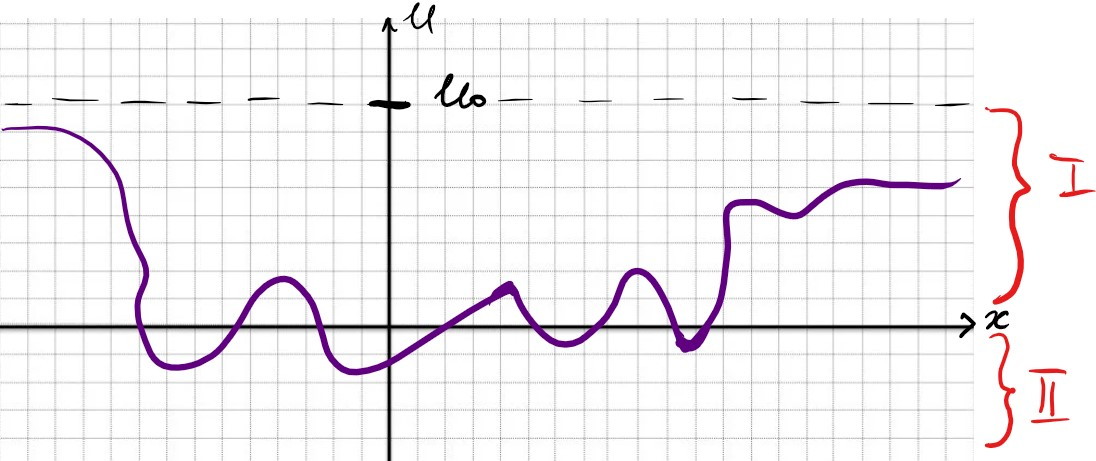
\includegraphics[width=1\linewidth]{pictures/20.1.jpg}
\caption{Классификация спектра}
\end{wrapfigure}
\par Область I на рисунке соответствует непрерывному спектру, но собственные значения $E_n$ не вырождены. Область II: $E<U$ асимптотически, спектр дискретный, в системе наблюдается затухание.
$$k=\sqrt{\frac{2mE}{\hbar^2}}$$
//много слов, есть парочка формул//
\par $\psi \rightarrow^{x \rightarrow \infty} a cos(kx+\delta) $, где $\delta$  - фаза рассеяния. Т.к. потока на бесконечности нет, там стенка потенциала (косинус выбрали, т.к. амплитуда упавшей и отраженной от стенки волн должны быть одинаковы).
\par При $x \rightarrow -\infty$ получим 
$$\psi\prime\prime - \frac{2m}{\hbar^2}(U_0 - E)\psi =0$$
\par Тогда $\psi = b e^{\kappa x}$, $\kappa = \frac{1}{\hbar}\sqrt{2m(U_0-E)}$ - затухание.
\par В неотмеченной области $E>U_0$ спектр непрерывный, но все уровни двухкратно вырождены. Оба независимых решения на бесконечностях удовлетворяют хорошим ГУ.
\par 5\textdegree. Если потенциал $U(x)$ - четная функция, то мы можем определить четность волновой функции. Итак, $\psi(x)$ - решение УШ
$$\hat{H}(x)\psi(x)=E\psi(x)$$
\par Сменим х на -х в этом уравнении
$$\hat{H}(-x)\psi(-x)=E\psi(-x)$$
\par Т.к. потенциал - функция четная, как и $\frac{\partial^2}{\partial x^2}$, то оператор Гамильтона не изменится, тогда $\psi(-x)$ - тоже решение УШ
$$\hat{H}(x)\psi(-x)=E\psi(-x)$$

\par Можем тогда сказать, что $\psi(-x)=C \psi(x)$, а если еще раз сменить -х на х, то получим еще одну связь $\psi(x)=C^2\psi(x)$ и константа $C=\pm 1$. Значит, \textit{все решенич есть четные или нечетные функции} и симметрия решения всегда меньше симметрии уравнения. Для основного состояния $\psi$-функция четная.

//+добавить этот же кусок в билет про четность состояния//
\par 6\textdegree. Нормировочный коэффициент непрерывного спектра
\par \textbf{a)} Рассмотрим волновую функция для движения, инфинитного в одну сторону $x \rightarrow \infty $. Нормировочный интеграл расходится на бесконечности, и это основной вклад в интеграл. Левый предел интегрирования можно выбрать любым образом. Пусть, например, x=0
$$\int \psi^*_p \psi_{p^\prime}dx = \delta \left( \frac{p-p^\prime}{2\pi \hbar}\right)$$
\par где р - импульс на бесконечности. При $x \rightarrow \infty$ имеем $\psi_p \approx  2 cos(kx+\delta)= e^{-i(kx+\delta)}+e^{i(kx+\delta)}$ - 2 стоячие волны. $p \rightarrow p\prime$, выкинем слагаемые с суммой $k$ и $k^\prime$, т.к. они не дадут $\delta$-функцию:
$$\int \psi^*_p \psi_{p^\prime}dx = \int^{\infty}_0 e^{i(k^\prime-k)x} dx + \int^{\infty}_0 e^{-i(k^\prime-k)x} dx = \int^{\infty}_{\infty} e^{i(k^\prime-k)x} dx $$
\par \textbf{б)} Переход к нормировке на $\delta$-функцию по энергии. Учтем в $\psi_p$:
$$\frac{d \left(\frac{p}{2\pi\hbar} \right)}{dE}^{\frac{1}{2}} = \frac{1}{\sqrt{2\pi\hbar V}} $$
$$\psi_E= \frac{\psi_p}{\sqrt{2\pi\hbar V}} = \frac{1}{\sqrt{2\pi\hbar V}} \left(e^{-i(kx+\delta)}+e^{i(kx+\delta)} \right)$$
\newpage
\chapter{Коэффициенты отражения и прохождения в одномерных задачах. Примеры}

\par 
\begin{wrapfigure}[9]{l}{0.25\linewidth} 
\vspace{-2ex}
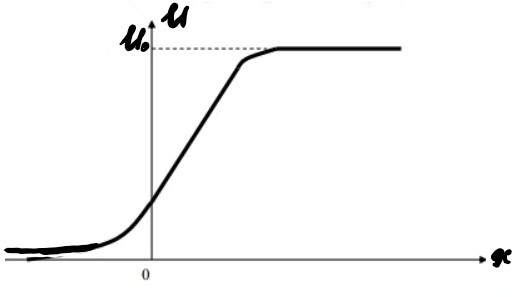
\includegraphics[width=1\linewidth]{pictures/21.1.jpg}
\caption{Вид рассматриваемого потенциала}
\end{wrapfigure}
\par При очень больших значениях $x\rightarrow \infty$ волновая функция будет выглядеть следующим образом (из граничных условий выбрали нулевой второй коэффициент) $\psi = A e^{ik_2x}$, где $k_2=\frac{1}{\hbar}\sqrt{2m(E-U_0)}$.
\par При отрицательных больших значениях $x\rightarrow -\infty$ получим с выбранным первым единичным коэффициентом: $\psi = e^{ik_1x} +B e^{-ik_1x} $, где $k_1 = \frac{1}{\hbar} \sqrt{2mE}$.
\par Плотность потока в падающей волне $k_1$, в отраженной $k_1|B|^2$, в прошедшей $k_2|A|^2$. Коэффициент прохождения $T=\frac{k_2}{k_1}|A|^2$, коэффициент отражения $R=B^2=1-T$.
\par Если дано произвольное стационарное состояние с E>$U_0$, зададим волновую функцию на $x=-\infty$ и $x=\infty$ соотвественно:
$$\psi=A_1 e^{ik_1x}+B_1 e^{-ik_1x} \text{, и }\psi=A_2 e^{ik_2x}+B_2 e^{-ik_2x}$$
\par Причем коэффициенты линейно связаны, т.к. представленные функции - это решение одного линейного лифференциального уравнения: $A_2=\alpha A_1+\beta B_1 $, где $\alpha $ и $\beta$ зависят от вида потенциала.
\par Знаем, что если $\psi$ - решение, то и $\psi^*$ тоже является решением (грубо говоря, мы инвертируем время $ t \rightarrow - t$):
$$\psi^*=A^*_1 e^{-ik_1x}+B^*_1 e^{ik_1x} \text{ при x} \rightarrow-\infty \text{, и при x} \rightarrow\infty\textit{ } \psi=A^*_2 e^{-ik_2x}+B^*_2 e^{ik_2x}$$
\par Роль $A_2$ теперь играет $B^*_2$, а т.к. это тоже решение, то можем определить связь коэффициентов:
$$B^*_2 = \alpha B^*_1 + \beta A^*_1 \textit{ или } B_2 = \alpha^* B_1 + \beta^* A_1$$
\par Постоянство потока даст $ k_1 (|A_1|^2 - |B_1|^2)=k_2 (|A_2|^2 - |B_2|^2)$ или $|\alpha|^2-|\beta|^2= \frac{k_1}{k_2}$.
\par Коэффициенты отражения совпадают при движении по и против оси Ох. Покажем это. Пусть $B_2=0$, тогда $\frac{B_1}{A_1}=-\frac{\beta^*}{\alpha^*}$ и коэффициент отражения слева $R_1 =|\frac{B_1}{A_1}|^2 = |\frac{\beta}{\alpha}|^2$. Теперь $A_1=0$ и $\frac{A_2}{B_2}=\frac{\beta}{\alpha^*}$, значит, коэффициент отражения справа $R_2 =|\frac{A_2}{B_2}|^2 = |\frac{\beta}{\alpha}|^2$, что мы и получали при вычислении коэффициента отражения слева.
\newpage
\chapter{Гармонический осциллятор}
\par Запишем оператор Гамильтона, выбрав коэффициенты в потенциале таким образом, что при записи уравнений Ньютона мы получим настоящий гармонический осциллятор с частотой $w$:
$$\hat{H}=\frac{\hat{\vec{p}}^2}{2m} +\frac{m w^2x^2}{2}$$
\par В УШ применим масштабное преобразование $x=y\cdot L$:
$$\left(-\frac{\hbar^2}{2m} \frac{\partial^2}{\partial x^2} + \frac{m w^2x^2}{2} \right) \psi = E \psi$$
$$\left(-\frac{\hbar^2}{2mL^2} \frac{\partial^2}{\partial y^2} + \frac{m w^2L^2}{2} y^2 \right) \psi = E \psi$$
$$\left(- \frac{\partial^2}{\partial y^2} + \frac{m w^2L^4}{\hbar^2} y^2 \right) \psi = \left( E \frac{2mL^2}{\hbar^2} \right)\psi$$
\par Хотим, чтобы $ \frac{m w^2L^4}{\hbar^2} =1$, а значит, $L = \sqrt{\frac{\hbar}{mw}}$ и $ E \frac{2mL^2}{\hbar^2} = E \frac{2}{\hbar w}$ - число, для нижнего уровня порядка единицы, тогда $E_{min}=\frac{\hbar w }{2}$. Итак,
$$E_{min} \sim \hbar w$$
\par Весь спектр дискретный, тогда решение ...
\par Найдем его двумя способами. 
\section{A. Матричный метод}
\par Уравнение движения $\hat{\ddot{x}} + w^2 \hat{x}=0$, запишем в матричном виде, здесь индексы отвечают каким-то базисным функциям:$(\ddot{x})_{mn} + w^2 x_{mn}=0$. Перейдем к такому набору, в котором базисные функции $\hat{H}$ диагонализуют его, обозначение не будем менять. Тогда
$$(\ddot{x})_{mn} = i w_{mn}(\dot{x})_{mn}=\left|\text{ здесь }w_{mn}=\frac{E_m-E_n}{t} \right|= - w^2_{mn}x_{mn}$$
\par Имеем $(w^2_{mn}-w^2)x_{mn} =0$, либо $x_{mn} =0$, либо $w_{mn}=\pm w$. Проведем нумеризацию состояний, т.ч. $\pm w$ будет соответствовать соседним уровням дискретного спектра $n \rightarrow n\mp 1$, т.е. $w_{n, n\mp1}=\pm w$. Не равны нулю только $x_{n, n\mp1}$.
\par Пусть волновая функция есть функция действительная, тогда из эрмитовости $\hat{x}^+=\hat{x}$ имеем $x_{mn}=x_{nm}$. Рассмотрим коммутатор $\hat{\dot{x}}$ и $\hat{{x}}$:
$$\hat{\dot{x}}\hat{{x}}- \hat{{x}}\hat{\dot{x}} = -i \frac{\hbar}{m} $$
$$(\dot{x} x)_{mn} - (x\dot{x} )_{mn}=-i \frac{\hbar}{m}  \delta_{mn}$$
\par $m=n$, $w_{ln}=-w_{nl}$
$$i \sum_l (w_{nl} x_{nl}x_{ln} - x_{nl}w_{ln}x_{ln})= 2 i \sum_l w_{nl}x^2_{nl} = -i \frac{\hbar}{m} $$
\par Пусть $l = n \pm 1$:
$$(x_{n+1, n})^2 - (x_{n, n-1})^2 = \frac{\hbar}{2mw}$$
\par Выберем $n=0$ для основного состояния, понятно, что $x_{0, -1}=0$. Сумма арифметической прогрессии даст
$$(x_{n, n-1})^2 =\frac{n \hbar}{2mw} \text{ } \rightarrow  \text{ } x_{n, n-1}=x_{n-1, n}= \sqrt{\frac{n \hbar}{2mw} }$$
\par Причем знак перед корнем - вопрос выбора системы функций.
$$H_{nn}=E_n=\frac{m}{2} \left((\dot{x}^2)_{nn}+w^2(x^2)_{nn} \right)= \frac{m}{2} \left(\sum_l i w_{nl}x_{nl}iw_{ln}x{ln}+w^2\sum_l x_{nl}x_{nl} \right)=$$
$$=\frac{m}{2} \sum_l (w^2+w^2_{nl})x^2_{ln} =\frac{m}{2} 2w^2 \left(\frac{n \hbar}{2mw} + \frac{(n+1) \hbar}{2mw} \right) = m \frac{\hbar}{2} (2n+1)=\hbar w \left(n + \frac{1}{2} \right), \text{ где } n = 0,1,2...$$
\par Получили искомый спектр 
\section{Б. Решение через УШ}
\par Запишем УШ
$$ \psi^{\prime\prime}_{yy} + \left(\frac{2E}{\hbar w} - y^2 \right) \psi =0$$
\par Вообще решением являются спецфункции - функции параболического цилиндра, но кто ж их запоминает для экзамена, будем смотреть асимптотики. При $y \rightarrow \infty$ уравнение принимает простой вид $ \psi^{\prime\prime} - y^2 \psi =0$, значит, в асимпотике решение будет содержать 
$$\psi = \upchi e^{-\frac{y^2}{2}}$$
\par Обозначим $\frac{2E}{\hbar w} -1 =2n$, тогда $\upchi^{\prime \prime}-2y \upchi^\prime +2n\upchi =0$. При $y \rightarrow \pm \infty $ $\upchi$ растет быстрее конечной степени у. Решение существует только для целых n. Область расходимости отодвигается как можно дольше, получаем сходящееся значения $\psi$(решение). Эти полиномы $\upchi$ есть \textbf{полиномы Эрмита $H_n(y)$}:
$$H_n(y) = (-1)^n e^{y^2} \frac{d^n}{dy^n}e^{-y^2}$$
\par С учетом нормировки получим решение 
$$\psi_n = \left( \frac{mw}{\pi \hbar} \right)^{\frac{1}{4}} \frac{1}{\sqrt{2^n n!}} exp \left(- \frac{mw}{2 \hbar} x^2 \right) H_n \left(x \sqrt{\frac{mw}{\hbar}} \right)$$
\par Основное состояние $n=0$: 
$$\psi_0 = \left( \frac{mw}{\pi \hbar} \right)^{\frac{1}{4}} exp \left(- \frac{mw}{2 \hbar} x^2 \right) $$
\par Рассмотрим оператор
$$\left(\hat{\dot{x}} - iw \hat{x} \right)_{n-1, n} = - \left(\hat{\dot{x}} + iw \hat{x} \right)_{n, n-1} = i \sqrt{\frac{2\hbar w n }{m}}$$
\par Т.к. $\psi_{-1}=0$, имеем $\left(\hat{\dot{x}} - iw \hat{x}\right) \psi_0 = 0 $ - дифференциальное уравнение на $\psi_0$. Подставляем $\hat{\dot{x}} = - i \frac{\hbar}{m} \frac{\partial}{\partial x}$:
$$\left(\hat{\dot{x}} + iw \hat{x}\right) \psi_{n-1} = \left(\hat{\dot{x}} + iw \hat{x}\right)_{n, n-1} \psi_{n}= i \sqrt{\frac{2w\hbar n}{m}} \psi_n $$
$$\psi_n = \underbrace{\sqrt{\frac{m}{2w\hbar n}} \left(-\frac{\hbar}{m}\frac{d}{dx}+wx \right)}_{\hat{a}^+} \psi_{n-1}$$
\par $\hat{a}^+$ есть \textbf{оператор рождения} кванта энергии в данном осцилляторе, можем таким же способом определить \textbf{оператор уничтожения} $\hat{a}^- \equiv \hat{a}$.
$$\hat{a}^+ = \sqrt{\frac{m}{2w\hbar n}} \left(-\frac{\hbar}{m}\frac{d}{dx}+wx \right) = \sqrt{\frac{m}{2w\hbar n}} \left(-i\frac{\hat{p}}{m}+wx \right) $$
$$\hat{a} = \sqrt{\frac{m}{2w\hbar n}} \left(\frac{\hbar}{m}\frac{d}{dx}+wx \right) $$
\par Если посчитать коммутатор ручками, получится, что $[\hat{a} \hat{a}^+]=1$. Так же можно записать оператор Гамильтона через данные операторы, причем $\hat{a}^+\hat{a}$ есть число квантов в одной моде:
$$\hat{H}= \hbar w \left(\hat{a}^+\hat{a} +\frac{1}{2} \right)$$
\newpage
\chapter{Квантовомеханическая частица в однородном электрическом поле}
\par Мы знаем, что на частицу с зарядом $e$ в электрическом поле действует сила $F=eE$, потенциал тогда $U=-Fx$. Запишем УШ
$$\psi^{\prime \prime} + \frac{2m}{\hbar^2} \left(E+ Fx \right) \psi =0 $$
\par В импульсном представлении ($\psi(x)\rightarrow a(p)$):
$$\hat{H} = \frac{p^2}{2m}-i\hbar F \frac{d}{dp}$$
$$ a(p) = \frac{1}{2\pi\hbar F} exp \left(\frac{i}{\hbar F} (Ep - \frac{p^3}{2m}) \right)$$
\par Обратным Фурье преобразованием найдем $\psi(x)$. Для этого обезразмерим уравнение, введя переменную
$$\xi = \left(x+\frac{E}{F} \right) \left(\frac{2mE}{\hbar^2} \right)^{1/3}$$
$$\psi^{\prime \prime} + \xi \psi =0$$
\par Опять решение выражается в спец-функциях - \textbf{функциях Эйри} $\Phi (\xi)$:
$$\psi(\xi) = A \Phi (-\xi) \text{, где } \Phi (\xi) = \frac{1}{\sqrt{\pi}} \int^{\infty}_0 cos \left(\frac{u^3}{3}+ u \xi \right) du$$
\par Рассмотрим асимптотики. При $\xi \rightarrow -\infty$ имеем $ \psi \rightarrow \frac{A}{2|\xi|^{1/4}} exp \left( - \frac{2}{3} |\xi|^{3/2} \right)$ - затухание. При $\xi \rightarrow \infty$ соответственно $\psi \rightarrow \frac{A}{|\xi|^{1/4}} sin \left( \frac{2}{3} \xi^{3/2}+\frac{\pi}{4} \right)$ - стоячая волна с переменной частотой. Нормировка на $\delta$-функцию $\int \psi(\xi)\psi(\xi^{\prime}) d\xi = \delta(E^{\prime}-E)$ даст полный ответ
$$\psi(\xi) = \frac{A}{2 \xi^{1/4}} \left(exp[i(\left(\frac{2}{3} \xi^{3/2}-\frac{\pi}{4} \right)] + exp[-i\left(\frac{2}{3} \xi^{3/2}-\frac{\pi}{4} \right)] \right) $$
\par Плотность потока в каждой волне 
$$V \left( \frac{A}{2 \xi^{1/4}}\right)^2 = \sqrt{\frac{2}{m}(E+Fx)}\left( \frac{A}{2 \xi^{1/4}}\right)^2 = A^2 \frac{(2\hbar F)^{}1/3}{4m^{2/3}}$$
\par Надо нормировать на... //послушать пару
\newpage
\chapter{Момент импульса}
\par //придется много слушать//
\section{Введение. Определение момента импульса}
\par Симметрия и изотропия пространства обеспечивают неизменность $\hat{H}$ при поворотах, откуда следует закон сохранения момента импульса. Введем $\delta \vec{\varphi}$ по оси вращения, тогда $\delta \vec{r_i} = [\delta \vec{\varphi}, \vec{r_i}]$.
$$\psi(\{\vec{r_i}+\delta \vec{r_i}\})= \psi(\vec{r_i})+\sum_i \delta r_i \nabla_i \psi = \underbrace{(1+\delta \vec{\varphi} \sum_i [r_i \nabla_i])}_{\text{оператор б.м. поворота}} \psi$$
$$\left[\sum_i [r_i \nabla_i], \hat{H}\right]=0$$
$$\hbar \hat{\vec{L}} = -i \hbar [\vec{r}\nabla]$$
$$\overline{\vec{L}}= -i \hbar \int \psi^+ \sum_i [r_i \nabla_i] \psi dq$$
\par В невырожденном стационарном состоянии $\overline{\vec{L}} = 0$, т.к. при инвертировании времени $t \rightarrow - t$ получим $\overline{L}=-\overline{L}$, откуда и выходит, что $\overline{L} = 0$.
\par Рассмотрим некоторые коммутаторы:
$$ [\hat{L}_i, \hat{x}_k]=i \varepsilon_{ikj}\hat{x}_j \text{,}\; [\hat{L}_i, \hat{p}_k] = i \varepsilon_{ikj}\hat{p}_j \text{,}\; [\hat{L}_i, \hat{L}_k] = i \varepsilon_{ikj}\hat{L}_j$$
\par Введем квадрат оператора момента импульса $\hat{\vec{L}}^2=\hat{L}^2_x+\hat{L}^2_y+\hat{L}^2_z$. Он одновременно измерим с каждой из компонент, т.е. $[\hat{\vec{L}}^2 L_i]=0$, $i=x,y,z$.
\par Другие удобные комбинации:
$$\hat{L}_{\pm}=\hat{L}_x\pm i \hat{L}_y, \; \; [\hat{L}_+\hat{L}_-]=2\hat{L}_z, \;\; [\hat{L}_z\hat{L}_-]=\hat{L}_-, \;\; [\hat{L}_z\hat{L}_+]=\hat{L}_+,\; \;$$
$$ \hat{\vec{L}}^2= \hat{L}_-\hat{L}_+ + \hat{L}^2_z+\hat{L}_z = \hat{L}_+\hat{L}_- + \hat{L}^2_z-\hat{L}_z$$
\par Рассмотрим сферические координаты:
\begin{equation*}
 \begin{cases}
    $$ x= r cos \varphi sin \theta $$
\\
    $$ y= r sin \varphi sin \theta $$ 
\\
    $$z= r cos \theta$$
 \end{cases}
\end{equation*}
\par Запишем наши операторы: $\hat{L}_z=-i \frac{\partial}{\partial \varphi}$, заметим, что $\hat{\vec{L}}^2$ практически представляет угловую часть лапласиана:
$$\hat{L}_{\pm} = e^{\pm i \varphi} \left(\pm \frac{\partial}{\partial \theta} + i ctg \theta \frac{\partial}{\partial \varphi} \right) \; \;\; \hat{\vec{L}}^2 = - \left(\frac{1}{sin^2\theta} \frac{\partial^2}{\partial \varphi^2} +\frac{1}{sin\theta} \frac{\partial}{\partial \theta}sin \theta \frac{\partial}{\partial \theta} \right)$$
\section{Собственные значения оператора $\hat{L}_z$}
$$-i \frac{\partial}{\partial \varphi} \psi = l_z \psi, \text{, откуда } \; \psi = f(r, \theta) e^{i l_z \varphi}$$
\par Из однозначности $\psi$-функции получаем, что $l_z = 0,\pm1, \pm2,...$.
\par Заметим, что $\Phi_m(\varphi) = \frac{1}{\sqrt{2\pi}} exp (im\varphi)$ и $\int^{2\pi}_0 \Phi^*_m(\varphi) \Phi_{m^\prime}(\varphi) d\varphi = \delta_{m m^\prime } $.
\section{Свойства}
\par 1\textdegree. $z \sim -z$, для любого собственного значения $l_z$ существует $-l_z$.
\par 2\textdegree. L - наибольшее возможное значение |M| (проекция).
$\hat{\vec{L}}^2 - \hat{L}^2_z = \hat{L}^2_x  + \hat{L}^2_y>0$, поэтому собственные значения $l_z$ ограничены сверху по модулю.
Если $\hat{L}_z\hat{L}_{\pm}\psi_M = (M \pm1) \hat{L}_{\pm} \psi_M $, то
\begin{equation*}
 \begin{cases}
    $$ \psi_{M+1} = const \hat{L}_{+} \psi_M $$
\\
    $$ \psi_{M-1} = const \hat{L}_{-} \psi_M $$ 
 \end{cases}
\end{equation*}
\par 3\textdegree. Т.к. не существует состояний с $M>l$, то $\hat{L}_+ \psi_l=0$.
$$\hat{L}_- \hat{L}_+ \psi_l = \left(\hat{\vec{L}}^2- \hat{L}^2_z-\hat{L}_z \right) \psi_l =0$$
\par \textbf{Собственные значения оператора}: $\hat{\vec{L}}^2\psi= l(l+1)\psi$, причем $M=l,l-1, ..., -l$. Итого $2l+1$ значений М.

\newpage
\chapter{Собственные функции момента импульса}
//здесь было много слов о полной системе измеримых физических величин//
\par Например, для $E=\frac{\vec{p}^2}{2m}$ есть $\hat{p}_x, \hat{p}_y, \hat{p}_z$  и все они меж собой коммутируют, каждый имеет свои собственные значения, определяющие энергию. В 1D 1 квантовое число ($p\equiv p_x$ - значит, одно собственное число), в 2D - 2, в 3D - 3. Мы рассматриваем 3D случай и у нас уже есть $\hat{L}_z$ и $\hat{L}^2$, не хватает еще одного оператора, и скорее всего эта третья физическая величина связана с радиальной компонентой.
\par Вспомним выражение $\hat{\vec{L}}^2=  \hat{L}_+\hat{L}_- + \hat{L}^2_z-\hat{L}_z$ и определим матричные элементы (первое слагаемое есть произведение двух матриц А и В, равное $\sum A_{ij}B_{jk}$)
$$l(l+1)= <M|\hat{L}_+|M-1><M-1|\hat{L}_-|M> + M^2 -M$$
\par Т.к. операторы $\hat{L}_+$ и $\hat{L}_-$ являются эрмитово сопряженными (из-за эрмитовости $\hat{L}_x$ и $\hat{L}_y$), то $<M-1|\hat{L}_-|M> = <M|\hat{L}_+|M-1>^*$, а значит, $|<M|\hat{L}_+|M-1>|^2=(l-M+1)(l+M)$ и 
$$<M|\hat{L}_+|M-1>|=<M-1|\hat{L}_-|M> = \sqrt{(l-M+1)(l+M)}$$
\par Знак перед корнем - это фаза выбранных собственных функций базиса, в котором мы работаем. Назовем собственные функции оператора $\hat{\vec{L}}^2$:
$$\int |Y_{lM}|^2 d \Omega = 1, \; d \Omega = sin \theta d\theta d\varphi$$
\par Выберем $Y_{lM} = \Phi_M(\varphi)F_{lM}(\theta)$, где $\Phi_M(\varphi)$ уже вывели, а значит, $\int^{\pi}_0 |F_{lM}|^2 sin\theta d \theta = 1$.
\par Запишем УШ для оператора $\hat{\vec{L}}^2$:
$$\frac{1}{sin^2\theta} \frac{\partial^2\psi}{\partial \varphi^2} +\frac{1}{sin\theta} \frac{\partial }{\partial \theta}sin \theta \frac{\partial \psi}{\partial \theta} +l(l+1)\psi =0$$
\par Решение содержит присоединенные полиномы Лежандра
$$F_{lM} = (-1)^M i^l \sqrt{\frac{2l+1}{2}\frac{(l-M)!}{(l+M)!}} P^M_l (cos\theta)$$
\par Как это вспомнить на экзамене? Никак. Подействуем оператором $\hat{L}_+$ на функцию $Y_{ll}$ или $\hat{L}_-$ на $Y_{l, -l}$, чтобы получить ноль:
$$\hat{L}_+Y_{ll} =0\; \rightarrow \; Y_{ll} = \frac{1}{2\pi} e^{il\varphi}F_{ll}(\theta)$$
\var Пользуемся оператором $\hat{L}_+$:
$$\frac{d F_{ll}}{d \theta} - l \cdot ctg \theta F_{ll}=0 \; \rightarrow \; F_{ll}= C sin^{l}x$$
\par Отсюда $F_{ll}= (-i)^l \sqrt{\frac{(2l+1)!}{2}} \frac{1}{2^ll!} sin^l \theta$. Шагаем вниз по правилу:
$$\hat{L}_- Y_{l, m+1}= \left(\hat{L}_- \right)_{m, m+1}Y_{l,m}= \sqrt{(l-m+1)(l-m)} Y_{lm}$$
\par Попозже напишу, откуда получаются следующие полезные формулы:
$$\sqrt{\frac{(l-m)!}{(l+m)!}}Y_{lm}= \frac{1}{\sqrt{(2l)!}} \hat{L}^{l-m}_- Y_{ll}$$
$$\hat{L}_- \left(f(\theta)e^{im\varphi} \right) = e^{-i(m-1)\varphi}sin^{l-1}\theta \hat{\vec{L}}^2 \psi = l(l+1) \psi$$
$$F_{lm}(\theta)= (-i)^l \sqrt{\frac{2l+1}{2}\frac{(l+M)!}{(l-M)!}} \frac{1}{2^l l! sin^m \theta} \frac{d^{l-m}}{(dcos\theta)^{l-m}} sin^{2l}\theta$$
\newpage
\chapter{Сложение моментов}
\par Пусть есть 2 слабовзаимодействующие системы с соответствующими моментами импульса, квантовыми числами и волновыми функциями:
\begin{table}[h]
\centering
\begin{tabular}[c]{|c|c|}
\hline 
1 подсистема & 2 подсистема \\ \hline 
$\hat{\vec{L}}^2_1$ и $\hat{\vec{L}}_{z1}$ & $\hat{\vec{L}}^2_2$ и  $\hat{\vec{L}}_{z2}$,\\
$L_1$ и $M_1$ & $L_2$ и $M_2$ \\
$\varphi_1(q_1)$ & $\varphi_2(q_2)$ \\
\hline
\end{tabular}
\end{table}
\par Масштаб для каждой из подсистем - расстояние между уровнями дискретного спектра. При взаимодействии уровни расходятся, появляются матричные элементы взаимодействия  $V_{nm}<< E_n -E_m$. Как сложить эти моменты? Можем определить оператор суммы и его квадрат, проекцию на $Oz$ (это направление не выделено, пространство изотропно, поэтому можно найти проекцию на совершенно любую ось): $\left(\hat{\vec{L}}_1 +\hat{\vec{L}}_2 \right)^2$. Тогда волновая функция $\varphi_{l_1, l_2, m_1, m_2}$ имеет $(2l_1+1)(2l_2+1)$ значений. Хотим перенумеровать, т.е. определить индексы, содержащие индексы полного момента.
$$\hat{\vec{L}}^2_1,\; \hat{\vec{L}}^2_{z2},\; \hat{\vec{L}}^2_1,\; \hat{\vec{L}}^2_{z2} \longrightarrow \varphi_{l_2l_2lm}$$
\par Причем $\varphi= \varphi_1(q_1) \cdot \varphi_2(q_2)$.
\par \textit{Небольшое отступление. Если $\hat{H}=\hat{H_1}(q_1)+\hat{H_2}(q_2)$, то УШ допускает разделение переменных: $\left( \hat{H_1}(q_1)+\hat{H_2}(q_2)\right)\varphi_1(q_1) \cdot \varphi_2(q_2) = E \varphi_1(q_1) \cdot \varphi_2(q_2) $ и соответственно $$\frac{\hat{H_1}(q_1)}{\varphi_1(q_1)} +\frac{\hat{H_2}(q_2)}{ \varphi_2(q_2)} = E$$
}
\par Можем сложить проекции моментов $\left(-i \hbar \frac{\partial}{\partial \varphi} \right)$.

\begin{table}[h]
\centering
\begin{tabular}[c]{|c|c|c|}
\hline 
M_1 & M_2 & M \\ \hline 
l_1 & l_2 & l_1+l_2\\
\begin{equation*}
 \begin{cases}
    l_1-1
\\
    l_1 
 \end{cases}
\end{equation*} & \begin{equation*}
 \begin{cases}
    l_2
\\
    l_2-1 
 \end{cases}
\end{equation*}&\begin{equation*}
 \begin{cases}
    l_1+l_2-1
\\
     l_1+l_2-1
 \end{cases}
\end{equation*}\\
...& ...& ...\\
\hline
\end{tabular}
\end{table}
\par Получается, одному значению суммарной проекции момента импульса могут соответствовать разные комбинации значений проекций моментов подсистем. При уменьшении $M$ таких комбинаций будет все больше.

\par 
\begin{wrapfigure}[10]{c}{0.45\linewidth} 
\vspace{-2ex}
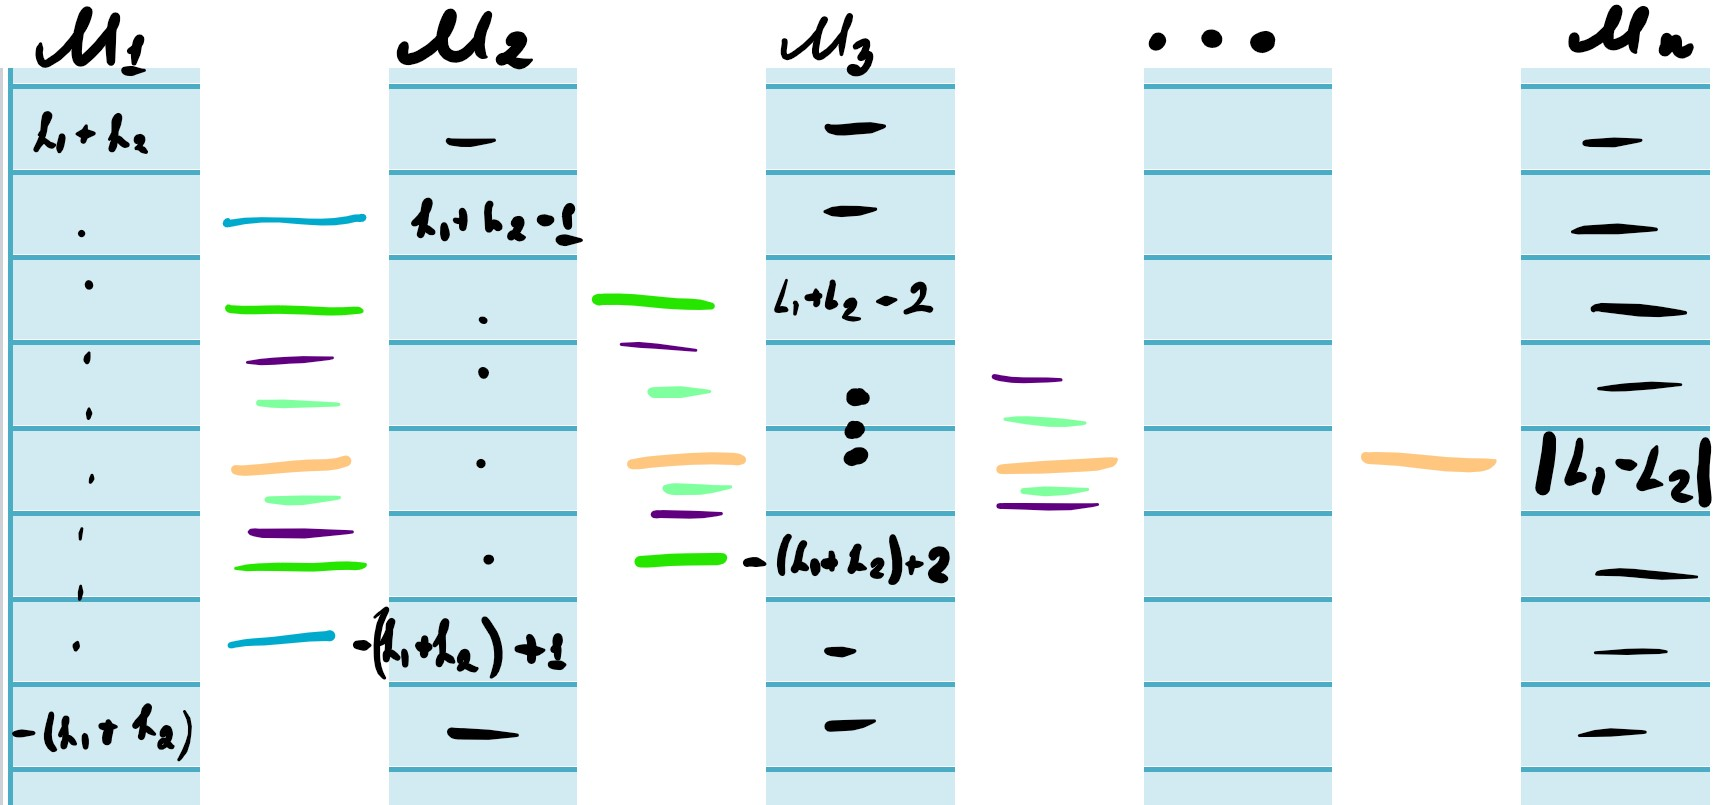
\includegraphics[width=1\linewidth]{pictures/18.1.jpg}
\caption{Увеличивающееся число комбинаций}
\end{wrapfigure}
\par Причем их число будет увеличиваться до тех пор, пока не останется суммарное значение $|l_1-l_2|$. Итого $l = \{ l_1+l_2,l_1+l_2-1, ..., |l_1-l_2|  \}$.
\par Итоговая четность состояния $(-1)^{l_{\sum}}$.
\newpage
\chapter{Частица в центральном поле}
\section{Общая задача взаимодействия двух частиц}
\par Запишем оператор Гамильтона для данной ситуации, пользуясь однородностью пространства: $\hat{H} = -\frac{\hbar^2}{2m_1} \frac{\partial^2}{\partial \vec{r_1}^2}-\frac{\hbar^2}{2m_2} \frac{\partial^2}{\partial \vec{r_2}^2} + U(|\vec{r_1}-\vec{r_2}|)$. Сведем к движению в центральном поле с помощью замены переменных и введения радиус-вектора центра масс: $\vec{r}=\vec{r_2}-\vec{r_1}$, $\vec{R}=\frac{m_1\vec{r_1}+m_2\vec{r_2}}{m_1+m_2}$, приведенная масса $\mu = \frac{m_1m_2}{m_1+m_2}$ Тогда //преобразования проделать ручками//
$$\hat{H}=-\frac{\hbar^2}{2(m_1+m_2)} \frac{\partial^2}{\partial \vec{R}^2} - \frac{\hbar^2}{2\mu} \frac{\partial^2}{\partial \vec{r}^2} + U(\vec{r})$$
\par Решаем УШ, ищем собственную функцию в виде $\Psi(\vec{r}, \vec{R})=\varphi(\vec{R})\psi(\vec{r})$:
$$-\psi \frac{\hbar^2}{2(m_1+m_2)} \frac{\partial^2\varphi}{\partial \vec{R}^2} -\varphi \frac{\hbar^2}{2\mu} \frac{\partial^2\psi }{\partial \vec{r}^2} + U(\vec{r}) = E$$
\par Разделяем переменные
$$\underbrace{-\frac{1}{\varphi} \frac{\hbar^2}{2(m_1+m_2)} \frac{\partial^2\varphi}{\partial \vec{R}^2}}_{\text{зависит только от } \vec{R}} \underbrace{-\frac{1}{\psi} \frac{\hbar^2}{2\mu} \frac{\partial^2\psi }{\partial \vec{r}^2} + U(\vec{r})}_{\text{только от } \vec{r}} = E$$
\par Тогда $-\frac{1}{\varphi} \frac{\hbar^2}{2(m_1+m_2)} \Delta \varphi = \varepsilon$ или $\varphi^{\prime \prime} +k^2 \varphi =0$, где $k^2=\frac{2(m_1+m_2)\varepsilon}{\hbar^2}$. Решение - $\varphi = A e^{i \vec{k}\vec{r}}+B e^{-i \vec{k}\vec{r}}$ - плоские волны.
\section{Частица в центральном поле}
\par Запишем оставшееся уравнение, учитывая, что энергия уже не та: $\Delta \psi +\frac{2m}{\hbar^2} (E-U)\psi = 0$ - это уравнение движение частицы в центральном поле. Записываем операторы в сферической СК и ищем решение в виде $\psi = R(r)\cdot Y_{lm}(\theta, \varphi)$.
$$ \frac{1}{r^2}\frac{\partial}{\partial r}\left(r^2  \frac{\partial \psi}{\partial r} \right) +\frac{1}{r^2} \left( \frac{1}{sin^2\theta} \frac{\partial^2\psi}{\partial \varphi^2} +\frac{1}{sin\theta} \frac{\partial }{\partial \theta}sin \theta \frac{\partial \psi}{\partial \theta}\right) +\frac{2m}{\hbar^2} (E-U)\psi =0$$

$$\frac{\hbar^2}{2m} \left(- \frac{1}{r^2}\frac{\partial}{\partial r}\left(r^2  \frac{\partial \psi}{\partial r} \right) + \frac{\hat{\vec{L}}^2}{r^2}\psi  \right) + U \psi = E \psi $$
$$\frac{\hbar^2}{2m} \left( - \frac{Y_{lm}}{r^2}\frac{\partial}{\partial r} \left(r^2  \frac{\partial R}{\partial r} \right) +  \frac{R}{r^2} l(l+1) Y_{lm} \right) + U RY_{lm}= E RY_{lm}$$
\par \begin{wrapfigure}[13]{r}{0.3\linewidth} 
\vspace{-2ex}
\centering
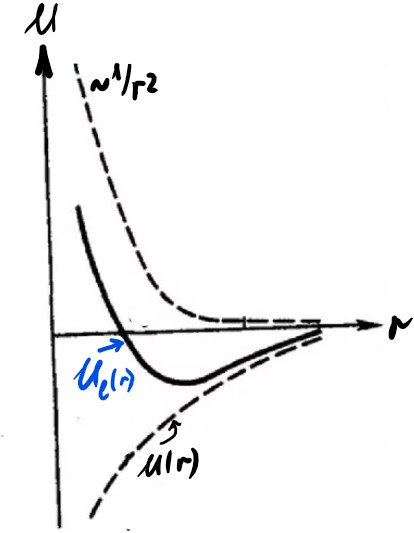
\includegraphics[width=1\linewidth]{pictures/27.1.jpg}
\caption{Измененный потенциал}
\end{wrapfigure}
\par Можем сократить сферические гармоники, получим
$$  \frac{1}{r^2}\frac{d}{d r} \left(r^2  \frac{d R}{d r} \right) -  \frac{l(l+1)}{r^2} R + \frac{2m}{\hbar^2} (E-U)R =0$$
\par Заменой $\chi = r R$ приводим к 
$$\chi^{\prime \prime}_{rr} + \left(\frac{2m}{\hbar^2} (E-U(r)) - \frac{l(l+1)}{r^2} \right) \chi =0$$

\par Задача определена на луче, требуем граничное условие $\chi(0) = 0 $, иначе получим расходимость в нуле для $R = \frac{\chi}{r}$.
\par Измененный потенциал $U_l (r) = U(r) + \frac{\hbar^2}{2m} \frac{l(l+1)}{r^2}$, где второе слагаемое описывает энергию вращения.
\par Уровни в потенциале нумеруются целыми числом $n_r$ - \textbf{квантовое радиальное число}. Кстати, полученные ранее числа $l$ и $m$ называются соответственно \textbf{квантовым азимутальным} и \textbf{квантовым магнитным числом}.
\par \begin{wrapfigure}[21]{l}{0.6\linewidth} 
\vspace{-2ex}
\centering
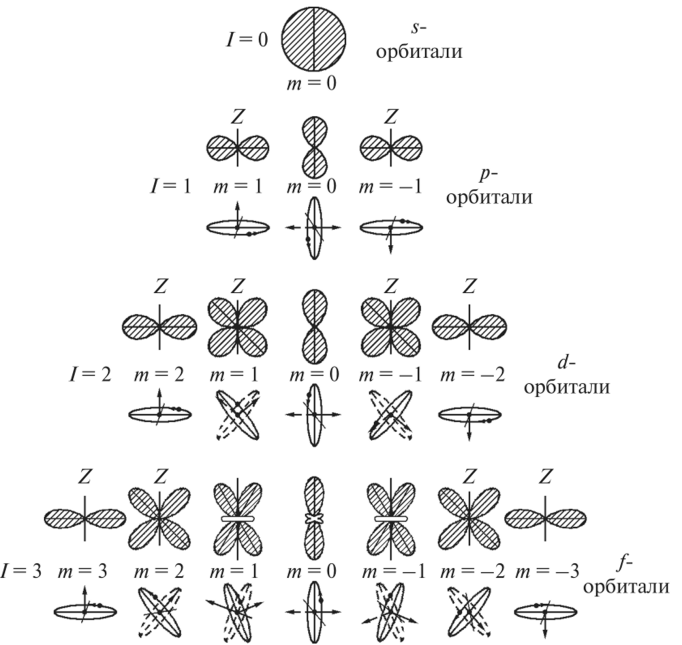
\includegraphics[width=1\linewidth]{pictures/27.2.png}
\caption{Атомные орбитали}
\end{wrapfigure}
\par Из атомной физики. Магнитное квантовое число m описывает ориентацию орбиталей в пространстве.
Для $l=0$ возможно только одно значение: $m=0$. Это значит, что s-орбиталь имеет только одну пространственную ориентацию.
Для $l=1$: $m=-1;0;+1$ - p-орбиталь имеет три пространственные ориентации.
Для $l=2$: $m=-2;-1;0;+1;+2$ - d-орбиталь имеет пять пространственных ориентаций.


\newpage
\chapter{Сферические волны}
\par Рассмотрим асимптотику в уравнении
$$  \frac{1}{r^2}\frac{d}{d r} \left(r^2  \frac{d R}{d r} \right) -  \frac{l(l+1)}{r^2} R + \frac{2m}{\hbar^2} (E-U)R =0$$
\par При $r\rightarrow 0$ обычно $\frac{d}{dx} \sim \frac{1}{x}$. И пусть $\lim\limits_{r \to 0}(U\cdot r^2)=0$. Тогда уравнение будет выглядеть следующим образом:
$$ \frac{1}{r^2}\frac{d}{d r} \left(r^2  \frac{d R}{d r} \right) -  \frac{l(l+1)}{r^2} R  =0$$
\par Решение его ищем в виде $R \sim r^s$: $s(s+1)=l(l+1)$, т.е. или $s=l$, или $s=-(l+1)$
\par При $r\rightarrow \infty$ и  $\lim\limits_{r \to \infty}(U)=0$ получим 
$$ \frac{1}{r^2}\frac{d}{d r} \left(r^2  \frac{d R}{d r} \right) -  \frac{l(l+1)}{r^2} R + \frac{2m}{\hbar^2} (E-\cancel{U})R =0$$
\par $E = \frac{\hbar^2}{2m}$. Получается задача о свободной частице с решением в виде плоских волн, спектр непрерывный (к - импульс плоских волн). Проблема в 3D - вырожденный спектр. 
\par Фактически, нам нужно перейти от плоских волн к сферическим. $\Delta \psi + k^2 \psi =0$ - решение есть потенциал сферического источника, при k=0 это $1/r$. Индексы: $k$ - модуль импульса, $l $- момент.
$$R^{\prime \prime}_{kl} + \frac{2}{r}R^\prime _{kl} +\left(k^2 - \frac{l(l+1)}{r^2} \right)R _{kl}=0$$
\par Нормировка $\int^\infty_0 r^\prime R_{k^\prime l}R_{kl}dr=2\pi \delta (k^\prime- k)$. Пусть $l=0$, тогда $R_{k0}= 2 \frac{sin kr}{r}$ (вообще перед $\frac{e^{\pm ikr}}{r}$ может быть любая константа, но именно двойка будет очень удобна). При $l \ne 0$ получим $R_{kl}= r^l \chi_{kl}(r)$. Уравнение на $\chi$:
$$\chi^{\prime \prime}_{kl} + \frac{2(l+1)}{r}\chi^{\prime}_{kl} + k^2 \chi_{kl} =0 $$
\par Продифференцируем его $\frac{\partial}{\partial r}$:
$$\chi^{\prime \prime \prime}_{kl}+ \frac{2(l+1)}{r}\chi^{\prime \prime}_{kl} + \left( k^2 - \frac{2(l+1)}{r^2} \right)\chi^{\prime}_{kl}=0 $$
\par Т.к. $\chi^{\prime}_{kl} = r \chi_{k,l+1}$, то, во-первых,
$$\chi^{\prime \prime \prime}_{kl}+ \frac{2(l+1)}{r}\chi^{\prime }_{k,l+1} +  k^2 \chi_{k,l+1}=0$$
\par И, во-вторых, $\chi_{kl}= \left(\frac{1}{r} \frac{d}{dr} \right)^l \chi_{k0}$. Получим $R_{kl} = (-1)^l 2 \frac{r^l}{k^l} \left(\frac{1}{r} \frac{d}{dr} \right)^l  \frac{sin kr}{r} = \sqrt{\frac{2 \pi k}{r}} J_{l+1/2}(kr)$ или же $R_{kl} = 2 k j_l(kr)$, где $j_l(kr)$ - сферическая функция Бесселя (или  функция Бесселя 2 рода).

\par \begin{wrapfigure}[5]{c}{1\linewidth} 
\vspace{-2ex}
\centering
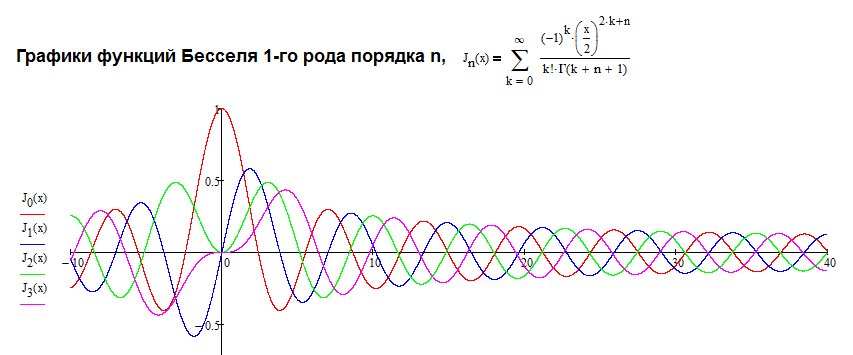
\includegraphics[width=1\linewidth]{pictures/28.1.png}
\caption{Функции Бесселя 1 рода}
\end{wrapfigure}

\par \begin{wrapfigure}[10]{r}{0.4\linewidth} 
\vspace{-2ex}
\centering
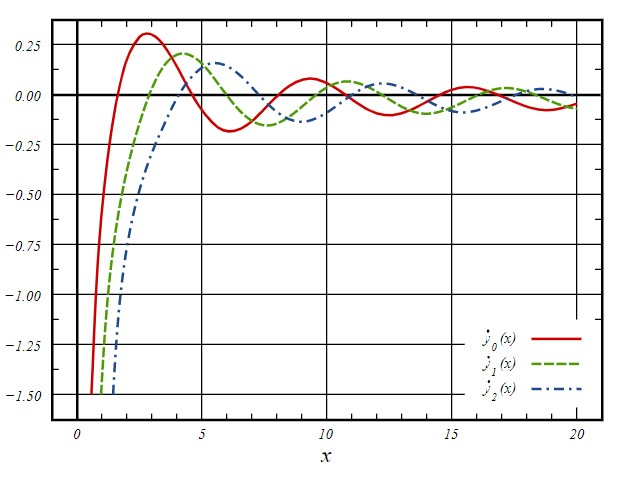
\includegraphics[width=1\linewidth]{pictures/28.2.jpg}
\caption{Функции Бесселя 2 рода}
\end{wrapfigure}
\par Асимптотики решения: $r \rightarrow \infty$ $R_{kl}\rightarrow \frac{2}{r} sin (kr- \pi l/2) $, при $ r \rightarrow 0$ $R_{kl}\rightarrow \frac{2k^{l+1}}{(2l+1)!!} r^l $.
\par $z = r cos \theta$: 
$$e^{ikz}=\sum^\infty_{l=0}(-i)^l(2l+1)P_l (cos\theta) \frac{r}{k}^l \left(\frac{1}{r} \frac{d}{dr} \right)^l  \frac{sin kr}{r}$$
\par $\forall \vec{k}$ можем выбрать ось $Oz$ и написать такое разложение, поэтому оно самого общего вида.
\newpage
\chapter{Частица в кулоновом поле. Уровни энергии и волновые функции}
\par Рассмотрим потенциал вида $U=-\alpha/r$, где $\alpha>0$. Для атома водорода $\alpha=E^2$. //куча слов о том, что невозможно отличить электроны друг от друга и про волновую функцию//
\par Запишем уравнение в таком потенциале (вывод см. в предыдущем билете):
$$R^{\prime \prime}_{kr} + \frac{2}{r}R^\prime _{r}  - \frac{l(l+1)}{r^2} R  +\frac{2m}{\hbar^2}\left( E+\frac{\alpha}{r}\right)R=0$$
\par Введем переменные для длины, времени и энергии для обезразмеривания уравнения: $L = \frac{\hbar^2}{m\alpha}$, $t=\frac{\hbar^2}{m\alpha^2}$, $[E] = \frac{m\alpha^2}{\hbar^2}$. Получим:
$$R^{\prime \prime}_{rr}+ \frac{2}{r}R^\prime _{r}   - \frac{l(l+1)}{r^2} R + 2\left(E+\frac{1}{r} \right)R $$
\par Пусть еще $r = \frac{1}{\sqrt{-2E}}$ и $\rho = \frac{2r}{n}$:
$$R^{\prime \prime} +\frac{2}{\rho} R^\prime + \left(-\frac{1}{4} + \frac{n}{\rho}-\frac{l(l+1)}{\rho^2} \right)R=0$$

\par \begin{wrapfigure}[15]{r}{0.5\linewidth} 
\vspace{-2ex}
\centering
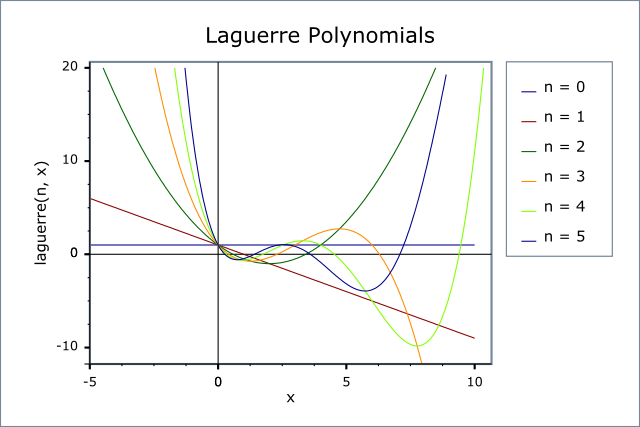
\includegraphics[width=1\linewidth]{pictures/29.1.png}
\caption{Полиномы Лагерра}
\end{wrapfigure}
\par Асимптотики: $\rho \rightarrow \infty$ и $R^{\prime \prime} -\frac{1}{4} R=0$, а значит, решение $R\rightarrow e^{-\rho/2}$ (знак выбран таким образом, что все затухает на бесконечности);$\rho \rightarrow 0$, попробуем подстановку $R=\rho^2 e^{-\rho/2} W(\rho)$:
$$\rho W^{\prime \prime} +(2l+2-\rho)W^\prime +(n-l-1)W =0$$
\par Решением являются спец-функции - \textbf{полиномы Лагерра}, причем должно выполняться условие $(n-l-1)\geq 0$, $n \in \mathds{Z}$. Получили энергию $E=-\frac{m \alpha^2}{2\hbar^2 n^2}$ с нижней границей $n \geq l+1$ , которая определяет \textbf{главное квантовое число}, связанное с  с радиальным и орбитальным квантовыми числами: $n_г = n-l-1$, оно равно числу узлов радиальной части волновой функции. Для любого n есть вырождение. //явно что-то говорил в этом месте//
\par Еще какие-то замечания, числа, формулы:
$\frac{\hbar^2}{ml^2}=0.8 \cdot 10^{-8} cm$ - пол-Ангстрема, боровский радиус;
$\frac{me^4}{\hbar^2}=27.21 эВ$ - масштаб/глубина энергии;
Число Ридберга - $R_y = 0.5 \frac{me^4}{\hbar^2}$
\par Число вырождения уровня при заданном $n$ и при $l=\{ 0,1,2,...,n-1\}$ равно $\sum^{n-1}_{l=0} (2l+1)=n^2$.
\newpage
\chapter{Калибровочное преобразование в квантовой механике}
\par Запишем УШ для ЭМ поля, учитывая $\vec{B} = rot\vec{A}$ и $ \vec{E}= - \nabla \varphi - \frac{1}{c} \frac{\partial \vec{A}}{\partial t}$:
$$\left(\frac{\left(\hat{\vec{p}} - \frac{e}{c} \vec{A}(\vec{r}) \right)^2}{2m} + U(\vec{r})\right) \psi = i \hbar \frac{\partial \psi}{\partial t}$$
\par Всегда можем положить 
\begin{equation*}
 \begin{cases}
    \vec{\widetilde{A}} = \vec{A} + \nabla f
\\
    \widetilde{\varphi} = \varphi - \frac{1}{c} \dot{f}
 \end{cases}
\end{equation*}
\par поля останутся прежними, но уравнения изменятся, вопрос в том, как добиться такого же уравнения. Попробуем преобразовать $\psi$-функцию, добавив фазу (дабы избежать изменения вероятности): $\psi = \widetilde{\psi} e^{i \alpha(\vec{r},t)}$. Подставим в Гамильтониан, сначала для одного действия оператора, а потом еще разок:
$$e^{i\alpha} \left(-i \hbar \nabla + \underline{\hbar \nabla \alpha} - \frac{e}{c} \vec{A} \underline{- \frac{e}{c} \nabla f }\right) \widetilde{\psi}$$
$$\left(-i \hbar \nabla + \hbar \nabla \alpha- \frac{e}{c} (\vec{\widetilde{A}} + \nabla f) \right)^2$$
\par Подчеркнутые слагаемые в сумме должны давать ноль, а значит, $\alpha= - \frac{ef}{\hbar c}$. Но тогда получается, что $\alpha$ - функция $f$ и дифференцировать ее нужно как сложную функцию, получим $\dot{\alpha}$, а если же потенциал взять в виде $U(\vec{r})= e \left(\widetilde{\varphi}-\frac{1}{c} \dot{f} \right)$, то и этот фактор сократится.
\par Пускай ничего не знаем про всякие калибровки, но у нас есть УШ и оно симметрично относительно локальных фазовых преобразований волновой функции. Но при подстановке уравнения изменились, т.к. про векторный потенциал мы ничего не знаем. Вводим ЭМ поле как компенсацию изменения волновой функции (результат требования симметрии). Такие поля называются \textbf{калибровочными полями}. Сам заряд $e$ получается так же как результат симметрии. 
//много слов, смысла мало//
\par Рассмотрим, в каком порядке нужно действовать операторами $\hat{\vec{p}}$ и $\hat{\vec{A}}$:
$$[\hat{\vec{p}}\hat{\vec{A}}]\psi = (\hat{\vec{p}}\hat{\vec{A}} - \hat{\vec{A}}\hat{\vec{p}})\psi = -i \hbar \nabla(\psi \vec{A})+i \hbar \vec{A} \nabla \psi = \left|\nabla(\psi \vec{A} ) = \vec{A} \nabla \psi - \psi div \vec{A} \right| = -i \hbar \psi div \vec{A}$$
\par Выбор $div \vec{A}$  и есть \textbf{калибровка}. Уровнения от калибровочных преобразований зависеть не должны, а значит, коммутатор вводить не стоит, оставляем в Гамильтониане комбинацию $\hat{\vec{p}} - \frac{e}{c} \vec{A}(\vec{r})$. 

\newpage
\chapter{Экспериментальные факты, указывающие на существование спина и внутреннего магнитного момента у электрона}
\par Мы познакомились с механическим моментом количества движения. Понятно, что с ним связан магнитный момент. Допустим, знаем токи, как тогда найти момент? По аналогии $\vb{r} \times \vb{j}$, это все идет из уравнений Максвелла: $rot \, \vb{B} = \frac{4 \pi}{c} \vb{j}$, предположим, что можно записать $\vb{j}=c \cdot rot \, \vb{M}$, откуда получим уравнение $rot \left( \vb{B} -4 \pi \vb{M} \right) = rot \, \vb{H} = 0$. Т.о. для нахождения момента по известному току, нужно записать УМ. Есть аналогичная задача - по известному току находится магнитное поле (закон Био-Савара-Лапласа), это и есть $\vb{r} \times \vb{j}$, в этом смысле задача не отличается ничем, кроме констант. Что любопытно: можем установить соотвествие проекции магнитного момента на механический момент (\textbf{гиромагнитное отношение}) для электрона 
$$\frac{M_z}{L_z} =\frac{e}{2mc}$$
\par \begin{remark}  Вычислим силу кругового тока, обусловленного движением электрона по круговой орбите. По определению, сила тока — это количество заряда, протекшего через поперечное сечение за единицу времени. В данном случае электрон за 1 секунду пересечет воображаемое сечение $\nu$ раз, где $\nu$ — частота вращения электрона. Поэтому имеем
$$I = e \nu = e \frac{1}{T} = \frac{e v}{2 \pi r}$$
\par Здесь $T$ - период вращения, а $v$ - линейная скорость электрона. Магнитный момент электрона, обусловленный вращением, равен
$$p_0 = I S = \frac{e}{t}\pi r^2= \frac{e v r}{2}$$
\par Направление вектора $\vb{p_0}$ определяется правилом правого винта. Данный магнитный момент принято называть \textit{орбитальным магнитным моментом электрона}. Движущийся по круговой орбите электрон обладает моментом импульса, который равен:
$$\vb{L_0} = \vb{r} \times m\vb{v}$$
\par Вектор $\vb{L_0}$ направлен противоположно вектору $\vb{p_0}$, а его величина с учетом связи линейной и угловой скоростей движения равна:
$$L_0 = rmv = rmwr = \m \frac{2\pi}{T}r^2 $$
\par Теперь можем найти соотношение, которое называется \textit{гиромагнитным (магнитомеханическим) отношением орбитальных моментов электрона}.
$$\frac{p_0}{L_0} = \frac{e}{2m}$$ 
\par Мы считали, что электрон движется по круговой орбите, но можно показать, что такое же соотношение справедливо и при движении электрона по эллиптической орбите. Гиромагнитное отношение указывает на наличие связи между магнитными и механическими свойствами магнетика. Действительно, если изменились его магнитные свойства, то это должно привести к изменению механических свойств. Справедливо и обратное — изменение механических свойств должно привести к намагничению магнетика. \textbf{Конец замечания.}
\end{remark}
\par Если мы перейдем к квантовой механике, $\vb{L}$ становится оператором $\hat{L}_z$, имеющий некоторый дискретный набор собственных значений, тогда естественно предположить, что с точностью до коэффициента $M_z$ повторяет $L_z$. Отсюда получим дискретные значения магнитного момента. 
\par Для проверки данных соображений в 1921 году Штерном и Герлахом был проведен следующий эксперимент.
\par \begin{wrapfigure}[13]{r}{0.45\linewidth} 
\vspace{-2ex}
\centering
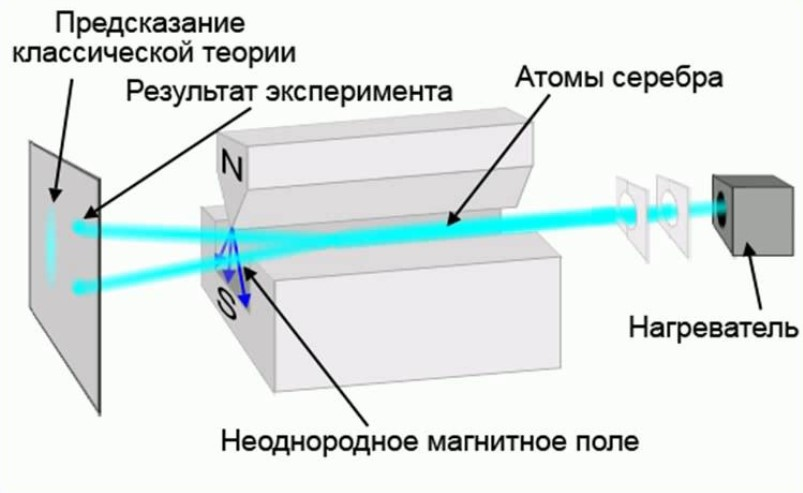
\includegraphics[width=1\linewidth]{pictures/31.1.jpg}
\caption{Опыт Штерна и Герлаха}
\end{wrapfigure}
\par Ставили экран с щелью, посылали на него пучок атома водорода (в оригинале - серебра) в s-состоянии (волновая функция изотропна, \textit{l=0}), далее была область неоднородного магнитного поля и ставили экран. Понятно, что энергия магнитного момента в магнитном поле $U=- \vb{M}\vb{B}$. Если $\vb{B}$ неоднородно, а $\vb{M}$ квантовано, то градиент потенциальной энергии даст силу, которая по-разному будет отклонять атомы, что даст какие-то дискретные следы на экране. В опыте получались 2 резких линии. Если бы это были классические частицы, мы бы получили некоторый разброс, но эта линия была бы одна и размытая. Вообще мы рассматриваем s-состояние, где нет орбитального и магнитного момента, о какой линии тогда может идти речь? Может, прогадали с условиями эксперимента, смотрим дальше: число проекций магнитного момента всегда нечетное (!), а получается явно две (!) полоски. Это был один из важных сигналов: волновая механика электрона в своей первоначальной форме не позволяет объяснить некоторых фактов магнитных и спектроскопических (см. далее) измерений.

\par Второй звоночек. В натрии изучали переход состоянии из $2p$ в $1s$ (первое число - это главное квантовое, s и p - квантовые). Увидели так называемый \textit{дублет} - две близкие линии. Опять возвращаемся к уже полученному противоречию. 
\par \begin{wrapfigure}[9]{l}{0.45\linewidth} 
\vspace{-2ex}
\centering
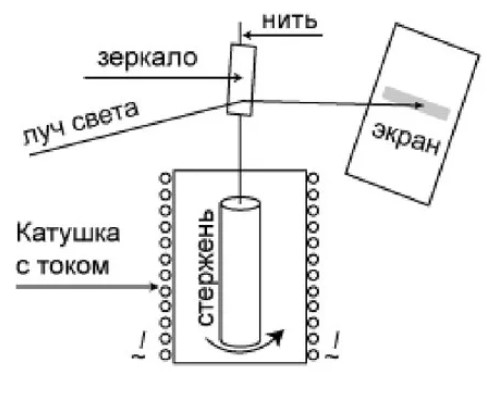
\includegraphics[width=0.7\linewidth]{pictures/31.2.jpg}
\caption{Опыт Эйнштейна-де-Гааза}
\end{wrapfigure}
\par Еще ранее, в 1915 году, был проведен еще один эксперимент - опыт Эйнштейна и Де Гааза

\par Тонкий железный стержень (ферромагнитный цилиндр) подвешивался на упругой нити и помещался внутрь соленоида. Для усиления эффекта применен метод резонанса - по соленоиду протекал переменный ток, частота которого подбиралась равной собственой частоте механических колебаний стержня. При намагничивании стержня магнитные моменты электронов установятся по направлению поля, а механические моменты против поля. В результате суммарный момент импульса электронов станет отличен от нуля. Момент импульса системы (стержень + электроны) должен остаться неизменным, поэтому стержень начнет закручиваться против вращения электронов. По измеренной амплитуде колебаний можно вычислить и механический момент, и гиромагнитное отношение, которое оказалось равным:
$$\frac{p_0}{L_0} = \frac{e}{m}$$
\par Отличие в 2 раза напрягало людей. В 1925 году Уленбек и Гоудсмит предположили, что у электрона, помимо того самого орбитального момента, который есть $\hbar m_z$, существует еще свой, \textbf{внутренний момент} - $S_z= \pm \hbar / 2$ и магнитный момент, который удовлетворяет гиромагнитному отношению без двойки. Проблема "полуцелых" состояний: выполнено условие невыделенности направления оси M (допустимые состояния -1/2 и 1/2), но волновая функция  $\psi$ этих состояний при повороте на $2\pi$ меняет знак, что на самом деле несколько тревожно. С другой стороны, нас интересует $|\psi|^2$, поэтому пока не будем обращать внимание на этот момент, посмотрим, что выйдет. Так появился \textbf{спин} - внутренний механический момент частицы.
\par Для спина собственных значений оператора $\hat{S}^2$ всего $s(s+1)$, для электрона $s=1/2$. Как ввести оператор спина - об этом и о других интересных фактах из жизни электрона смотри в следующем семестре.
\newpage
\chapter{Оператор спина. Уравнение Паули (нет в билетах этого года)}
\par По курсу еще не дошли до данной темы.
\par Спиновое квантовое число $m_s$ описывает направление вращения электрона в магнитном поле - по часовой стрелке или против. На каждой орбитали может находиться только два электрона: один со спином +½ другой -½.
Квантовые числа для первых трех энергетических уровней:

На первом уровне (n=1) есть только s-орбиталь, на которой может находиться только 2 электрона со спинами +1/2 и -1/2. Это справедливо для s-орбитали любого уровня: 1s; 2s; 3s…

На втором энергетическом уровне (n=2) есть уже две орбитали s; p. 
На третьем (n=3) - три орбитали: s, p, d. и т.д. С каждым новым энергетическим уровнем добавляется новая орбиталь.

Для 2p-орбитали существует три пространственных ориентации (формы облака), на каждой из которых может находиться по два электрона. Т.е. на втором энергетическом может находиться не более 6 p-электронов.

Для 3d - максимум 10 d-электронов и пять форм облаков.

Главные энергетические уровни отличаются энергией. Чем выше уровень - тем выше энергия. С другой стороны, различные орбитали одного и того же уровня также обладают разной энергией:
Энергия электронов на орбитали 2p выше, чем на 2s
Энергия электронов на орбитали 3p выше, чем на 3s
Энергия электронов на орбитали 3d выше, чем на 3s
Энергия электронов на орбитали 3d выше, чем на 3p
Что же касается электронов "внутри орбиталей", то их энергии одинаковы.

\par Принцип Паули: электроны располагаются так, что каждый из них имеет строго определённый набор квантовых чисел, в атоме не может быть даже двух электроновсо всеми четырьмя одинаковыми квантовыми числами.

Правило Хунда определяет порядок заполнения орбиталей определённого подслоя и формулируется следующим образом: модуль суммарного значения спинового-квантового числа электронов данного подслоя должен быть максимальным.

Это означает, что в каждой из орбиталей подслоя заполняется сначала один электрон, а только после исчерпания незаполненных орбиталей на эту орбиталь добавляется второй электрон.
\newpage
\chapter{Заряженная частица в однородном магнитном поле}
\par  Рассмотрим задачу о постоянном однородном электромагнитном поле. Нужно найти $\psi$ и $E$:
$$\frac{\left(\hat{\vec{p}} - \frac{e}{c} \vec{A}(\vec{r}) \right)^2}{2m}  \psi = E \psi$$
\par \textbf{1. Ищем векторный потенциал.} $\vec{B}= \mu \vec{H}$, $\vec{H} \uparrow \uparrow \vec{z}$.
\par
$$rot \vec{A} = \left |\begin{matrix} \vec{x}_0 & \vec{y}_0 &\vec{z}_0  \\ \frac{\partial}{\partial x} & \frac{\partial}{\partial y} &\frac{\partial}{\partial z} \\ A_x & A_y & A_z \end{matrix} \right| = \vec{x}_0 \left(\frac{\partial}{\partial y}A_z - \frac{\partial}{\partial z} A_y\right) -  \vec{y}_0 \left(\frac{\partial}{\partial x} A_z - \frac{\partial}{\partial z}A_x  \right) + \vec{z}_0 \left(\frac{\partial}{\partial x}A_y -  \frac{\partial}{\partial y}A_x   \right) $$
\par Т.к. $\vec{B}$ имеет только одну компоненту, то $$\frac{\partial}{\partial y}A_z - \frac{\partial}{\partial z} A_y = 0 \qquad \frac{\partial}{\partial x} A_z - \frac{\partial}{\partial z}A_x  = 0 \qquad \frac{\partial}{\partial x}A_y -  \frac{\partial}{\partial y}A_x  = B_z$$
\par 
\begin{wrapfigure}[18]{r}{0.4\linewidth} 
\vspace{-2ex}
\centering
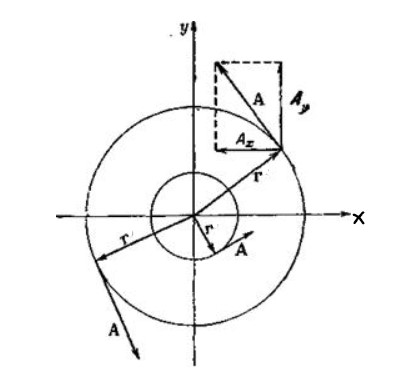
\includegraphics[width=1\linewidth]{pictures/30.1.jpg}
\caption{Однородное магнитное поле $\vec{B}$, направленное по оси $Oz$, соответствует векторному потенциалу $A_{\theta}= \frac{1}{2} rH$, который вращается вокруг этой оси. $r$ - расстояние до оси $Oz$.}
\end{wrapfigure}
\par Тогда можем взять $\vec{A} = \frac{1}{2}(-y, x, 0)H$. Поскольку x-компонента пропорциональна -y, а y-компонента пропорциональна x, то вектор  должен быть перпендикулярен вектору $\vec{r}$, проведенному от оси $Oz$. Кроме того, величина $\vec{A}$ пропорциональна $\sqrt{x^2+y^2}$ и, следовательно, пропорциональна $\vec{r}$. Поэтому для однородного поля можно записать $\vec{A}= \frac{1}{2} \vec{B} \times \vec{r}$ или же $A_{\theta}= \frac{1}{2} rH$ (\textbf{радиальная калибровка}). Векторный потенциал  вращается вокруг оси $Oz$, как показано на рисунке 30.1. Если, например, поле $\vec{B}$ есть поле внутри соленоида вдоль его оси, то векторный потенциал циркулирует точно таким же образом, как и токи в соленоиде.
\par Выберем калибровку $\vec{A} = (-y, 0, 0)H$.
\par \textbf{2. Распишем уравнение покомпонентно.}
$$\frac{\left(-i\hbar \frac{\partial}{\partial x} - \frac{e}{c}(-Hy) \right)^2}{2m}\psi - \frac{\hbar^2}{2m} \frac{\partial^2}{\partial y^2}\psi - \frac{\hbar^2}{2m} \frac{\partial^2}{\partial z^2}\psi =E \psi$$
\par Избавимся от производной по $z$: $\frac{(p_z)^2}{2m}$ - кинетическая энергия вдоль поля, частица не испытывает влияния, но в классике действует сила Лоренца и частица движется по окружности.
\par В уравнении нет в явном виде координат $x$ и $z$ - они циклические, значит, можем произвести разделение переменных, введя замену (а после опустить волну в уравнении):
$$ \psi = \widetilde{\psi} e^{i k_z z}e^{i k_x x} $$
$$\frac{1}{2m} \underbrace{\left(\hbar k_x + \frac{eH}{c} y \right)^2}_{U} \psi - \frac{\hbar^2}{2m} \frac{\partial^2 \psi}{\partial y^2} = \left(E - \frac{\hbar^2 k^2_z}{2m} \right) \psi$$
\par где $U$ - потенциал гармонического осциллятора со смещенной координатой $y$ на $const$.
$$\psi^{\prime \prime} + \frac{2m}{\hbar^2} \left(\left(E- \frac{p^2_z}{2m} \right) - \frac{m}{2} w^2_H (y-y_0)^2 \right) \psi = 0$$
\par Здесь $y_0 = -\frac{c p_x}{eH}$ - положение центра орбиты, $e=-|e|$ - заряд электрона, $w_H = \frac{|e|H}{mc}$ - циклотронная частота. Спектр осциллятора: 
$$E= \frac{p^2_z}{2m} +\hbar w_H (n+1/2)$$ 
\par Это \textbf{уровень Ландау}. В 1930 году эту задачу решил Ландау (хотя Фок сделал это раньше), он  вычислил измеримые величины (сказал, что диамагнетизм системы подвижных носителей зарядов связан с тем, что при помещении заряженных частиц в магнитном поле траектории свободного движения частиц искривляются и возникает добавочное магнитное поле, противоположное внешнему, т. е. у системы заряженных частиц появляется добавочный диамагнитный момент. Этот диамагнетизм заметно проявляется при низких температурах (ниже температуры вырождения) и может наблюдаться в вырожденном газе свободных электронов и у электронов проводимости в металлах, полуметаллах и полупроводниках). 
\par Решение полученного дифференциального уравнение дается спец-функциями - функциями Эрмита: $\psi = \Phi \left(\frac{y-y_0}{L_H} \right)$, где $L_H= \sqrt{\frac{\hbar c}{eH}}$ - магнитная длина.
\par //куча слов//
\par Тот факт, что энергия не зависит от $p_x$ ($k_x$) означает, что данные состояния вырождены, причем вырождение бесконечно-кратное. Куда делось движение по окружности при $\hbar \rightarrow 0 $ - исчезла калибровочная инвариантность.

\par //Наверное, надо еще включить все остальное про ток, связанный с квантовомеханическим электроном, и про вывод плотности потока вероятности...//


\newpage

\chapter{То что знали, но всегда хотели узнать}
\par Разные интересные факты и их доказательства, а также расписанный ход мысли. Данная глава выступает всеобщим протестом против слов: очевидно, не трудно показать и тд...
\section{Какой знак правильный?}
\par Старый пряник однажды спросил у хорошего, но малознающего студента: \textit{Почему у Вас уравнение Шрёдингера написано так: $ \mathfrak{ -i h \frac{\partial \psi(t)}{\partial t} = \hat{H}\psi } $}. Не очевидно, что принято записывать уравнение Шрёдингера так: $ \mathfrak{ i h \frac{\partial \psi}{\partial t} = \hat{H}\psi } $.
\par На самом деле обе записи верны: сменой направления течения времени они сводятся друг к другу, то есть при замене $\mathfrak{t \rightarrow -t}$. Напомню, проблема с течением времени решается лишь только в некоторых областях физики при помощи добавления вероятности происхождения того или иного события, а также при помощи причнно-следственной связи.
\section{Преподаватель на зачёте был не нужен}
\par Все совпадения с реальными зачётами, где студенты понимали вопрос преподавателя, искажая его смысл, остаются глубоко в душе и требуют ответа. Тема этой секции - уравнение непрерывности: $$\mathfrak{\frac{\partial |\psi|^2 }{\partial t} + div \! \left( \ \! \vec{j} \ \! \right) = 0 }$$
\begin{center}
    \textit{ Как вывести в общем виде, что $\mathfrak{\frac{\partial |\psi|^2 }{\partial t}}$ это есть дивергенция какого-то вектора и только? } 
\end{center}
\par Прежде чем решать такую сложную и общую задачу надо пытаться решать для более простой с гамильтанианом частного вида: $\mathfrak{ \hat{H} = \frac{\hat{p}^2}{2m}}$. При решении можно получить следующие важные сведения: во-первых, от импульса $\mathfrak{\hat{\vec{p}} = -i h \vec{\nabla}} $ нам важно  $\mathfrak{\hat{\vec{p}} \sim \vec{\nabla}}$, поэтому для вывода уравнения непрерывности нам нужно следить за степенями $\mathfrak{\hat{\vec{p}}}$. Во-вторых, Гамильтониан применённый к пси функции должен выдавать скаляр умноженный на пси функцию, никак не вектор, следствием этого будет требование некторых констант быть векторами. Из сказанного выше выпишем гамильтаниан общего вида, разложив его в полином от, учитывая что комутатор импульса и константа перед ними не коммутируют: $\mathfrak{\hat{\vec{p}}}$:
$$ \mathfrak{ \hat{H} = \sum_{s=0}^{k} A_s  \hat{\vec{p}}^{ \ s} + \sum_{s=0}^{k}  \hat{\vec{p}}^{ \ s} B_s  }  $$
Для нечётных $\mathfrak{s}$ важное свойство $\mathfrak{A_s}$: $ \mathfrak{ A_{2n+1} \equiv{} \vec{A}_{2n+1}}$. Приведу вывод для коэффициентов, хотя, зная вид оператора импульса, можно сказать, что это уже было выведено. Воспользуемся знанием, что $\mathfrak{\hat{{H}}}$ - эрмитов оператор: $\mathfrak{ \left(  \hat{H} \psi, \psi \right) = \left( \psi, \hat{H} \psi \right)} $
 $$ \mathfrak{ \left(   \psi, \hat{H} \psi \right) = \int \psi^* \hat{H} \psi \ dq = \int \psi^* \left( \sum_{s=0}^{k} A_s   \hat{\vec{p}}^{ \ s} \right)  \psi \ dq  =A_0 \int |\psi|^2 \ dq + \int \psi^* \left( \sum_{s=1}^{k} A_s   \hat{\vec{p}}^{ \ s} \right)  \psi \ dq} = $$
 $$ \mathfrak{ = A_0 + \int \psi^* \left( \sum_{s=0}^{k-1} A_{s+1}   \hat{\vec{p}}^{ \ s+1} \right)  \psi \ dq = A_0 + \int \psi^* \hat{\vec{p}}  \left( \sum_{s=0}^{k-1} A_{s+1}   \hat{\vec{p}}^{ \ s} \right)  \psi \ dq }$$
\par Далее потребуется воспользовать знанием что импульс это $\vec{\nabla}$ тогда можно записать подытегральную функцию как $ \mathfrak{\nabla \left( \psi^* \left( \sum_{s=0}^{k-1} A_{s+1}   \hat{\vec{p}}^{ \ s} \right)  \psi \right) - \hat{\vec{p}} \psi^*   \left( \sum_{s=0}^{k-1} A_{s+1}   \hat{\vec{p}}^{ \ s} \right)  \psi }$. По теореме Остроградского-Гаусса получим:
$$ \mathfrak{ A_0 + \oint \psi^* \left( \sum_{s=0}^{k-1} A_{s+1}   \hat{\vec{p}}^{ \ s} \right)  \psi \ dS - \int \hat{\vec{p}} \psi^*   \left( \sum_{s=0}^{k-1} A_{s+1}   \hat{\vec{p}}^{ \ s} \right)  \psi \ dq  = A_0 - A_1 \int \hat{\vec{p}} \psi^* \psi \ dq - } $$
$$ \mathfrak{ - \int \hat{\vec{p}} \psi^*   \left( \sum_{s=0}^{k-2} A_{s+2}   \hat{\vec{p}}^{ \ s+1} \right)  \psi \ dq }$$
\par Далее действуем аналогично и получаем при некоторых условиях (чтобы интегралы по замкнутым поверхностям были нулями) получаем следующую формулу:
$$ \mathfrak{\int \psi^* \left( \sum_{s=0}^{k} A_s   \hat{\vec{p}}^{ \ s} \right)  \psi \ dq = \int \psi \left( \sum_{s=0}^{k} (-1)^s A_s    \hat{\vec{p}}^{ \ s} \right) \psi^*  \ dq} $$
\par из определения сопряженного оператора следует, что справа написан комплексно сопряжённый оператор к $\mathfrak{\hat{H}}$, поэтому $\mathfrak{ \sum_{s=0}^{k} A_s^*   \hat{\vec{p}}^{*  s} = \sum_{s=0}^{k} (-1)^s A_s \hat{\vec{p}}^{ \ s} }$. Делаем вывод - определённый нами оператор импульса подходит под данных критерий, т.к. все его чётные степени при комплексном сопряженнии не меняют знак, а нечётные - меняют. Определив так импульс, мы требуем от чисел (векторов) $\mathfrak{A_s}$ действительность. Аналагично проделаем тоже самое с другой частью, в  выводе главное следить за порядком действия $\mathfrak{ B}$ и $\mathfrak{ \hat{\vec{p}} }$.  Сейчас у нас всё готово для доказательства в силу уравнения Шрёдингера:
$$ \mathfrak{ \frac{\partial |\psi|^2 }{\partial t} = \psi \frac{\partial \psi^*}{\partial t} + \psi^* \frac{\partial \psi}{\partial t} = \frac{i}{h} \left(  \psi^* \hat{H} \psi - \psi \hat{H}^* \psi^* \right)} $$
\par Из эрмитовости $\mathfrak{\hat{H}}$ (для проверки припишите слева ещё одну волновую функцию и воспользуйтесь определением сопряжённого оператора) получим:
$$ \mathfrak{ \frac{i}{h} \left(  \psi^* \hat{H} \psi - \psi \hat{H}^* \psi^* \right) = }$$
\par Из-за множителя $\mathfrak{(-1)^s}$ Останутся лишь нечётные элементы ряда, которые удвоятся. Выделим один $\mathfrak{\hat{\vec{p}}}$ и распишем его через оператор набла, не забудем что нечётные $\mathfrak{A_s}$ - действительные вектора , результат: ($\mathfrak{[x]}$ - целая часть числа $\mathfrak{x}$)
$$ \mathfrak{ 2 \vec{\nabla} \left( \sum_{s=0}^{[\frac{k-1}{2}]} \vec{A_{2s+1}} \hat{\vec{p}}^{ \ 2s} |\psi|^2 \right)  \equiv -div \! \left( \ \! \vec{j} \ \! \right) } $$
$$ \mathfrak{ \vec{j} = -2 \sum_{s=0}^{[\frac{k-1}{2}]} \vec{A_{2s+1}} \hat{\vec{p}}^{ \ 2s} |\psi|^2  } $$
\par {\gothfamily Kvant Mech}




\end{document}
